\documentclass[letterpaper,12pt]{article}

% Load packages
% - See complete list of packages at: https://www.ctan.org/pkg/
\usepackage[left=1in,right=1in,top=1in]{geometry}
\usepackage{graphicx}					% Enhanced support for graphics
\usepackage{float}						% Improved interface for floating objects
\usepackage{amsmath}					% AMS mathematical facilities for Latex
\usepackage{enumitem}					% Control layout of itemize, enumerate, description
\usepackage{cite}						% Improved citation handling in Latex
\usepackage{mathtools}					% Mathematical tools to use with amsmath
\usepackage{color}						% Colour control for Latex documents
\usepackage[makeroom]{cancel}			% Place lines through maths formulae
\usepackage{soul}						% Hyphenation for letterspacing, underlining, and more
\usepackage{dashbox}					% Draw dashed boxes
\usepackage{microtype}					% Subliminal refinements towards typographical perfection
\usepackage[table]{xcolor}				% Driver-independent color extensions for Latex and PDFLatex
\usepackage{subcaption}					% Support for sub-captions
\usepackage{longtable}					% Allow tables to flow over page boundaries
\usepackage{listings}					% Typeset source code listings using Latex
\usepackage[colorlinks=false,pdfborder={0 0 0}]{hyperref}	% Extensive support for hypertext

% For figures
\restylefloat{figure}					% To re-style the 'figure' float

% Path for graphics/figures
\graphicspath{{./Figures/}
			  {./Figures/Obj_BG_Cam/}}	% Location folder of all figures in paper


% For quotes
\usepackage{setspace}					% Set space between lines
\usepackage{etoolbox}					% e-Tex tools for Latex
\AtBeginEnvironment{quote}{\singlespacing\small}

% New commands to keep things shorter in document
\newcommand\dboxed[1]{\dbox{\ensuremath{#1}}}
\newcommand{\volume}{\mathop{\ooalign{\hfil$V$\hfil\cr\kern0.08em--\hfil\cr}}\nolimits}
\newcommand{\HRule}{\rule{\linewidth}{0.5mm}} 	% Defines a new command for the horizontal lines

% Define colors for code
\definecolor{mygreen}{RGB}{28,172,0}
\definecolor{mylilas}{RGB}{170,55,241}
\definecolor{mGreen}{rgb}{0,0.6,0}
\definecolor{mGray}{rgb}{0.5,0.5,0.5}
\definecolor{mPurple}{rgb}{0.58,0,0.82}
\definecolor{backgroundColour}{rgb}{0.95,0.95,0.92}
\definecolor{myMagenta}{rgb}{0.8,0,0.4}
\definecolor{myBlue}{rgb}{0, 0.4470, 0.7410}

\lstdefinestyle{C}
{
    backgroundcolor=\color{backgroundColour},   
    commentstyle=\color{mGreen},
    keywordstyle=\color{magenta},
    numberstyle=\tiny\color{mGray},
    stringstyle=\color{mPurple},
    basicstyle=\footnotesize,
    breakatwhitespace=false,         
    breaklines=true,                 
    captionpos=b,                    
    keepspaces=true,                 
    numbers=left,                    
    numbersep=5pt,                  
    showspaces=false,                
    showstringspaces=false,
    showtabs=false,                  
    tabsize=2,
    language=C
}

\lstdefinestyle{MATLAB}
{
    %basicstyle       = \tiny,
    %basicstyle		 = \ttfamily,
    %basicstyle       = \normalsize\fontencoding{T1}\ttfamily,
    breaklines       = true,
    morekeywords     = {matlab2tikz},
    keywordstyle     = \color{blue},
    morekeywords     = [2]{1},
    keywordstyle     = [2]{\color{black}},
    identifierstyle  = \color{black},
    stringstyle      = \color{mylilas},
    commentstyle     = \color{mygreen},
    showstringspaces = false,					% Without this, symbol in place of spaces
    numbers          = left,
    numberstyle      = {\tiny \color{black}},	% size of the numbers
    numbersep        = 9pt, 					% This defines how far the numbers are from the text
    emph             = [1]{for,end,break}
    emphstyle        = [1]\color{red},
    tabsize          = 4
}

\lstdefinestyle{CMD}
{
    backgroundcolor=\color{black},
    basicstyle=\normalsize\color{white}\ttfamily
}

% Begin the documents
\begin{document}

\begin{titlepage}

%\newcommand{\HRule}{\rule{\linewidth}{0.5mm}} 	% Defines a new command for the horizontal lines, change thickness here

% Center everything on the page
\center

% Show the title
\HRule \\[0.6cm]
{ \huge \textbf{How To Take Pictures Like NASA} \\[0.4cm] \textit{DIY Background Oriented Schlieren}}\\[0.4cm]
\HRule \\[1.5cm]

% Show the author
\Large \emph{Author:}\\
JoshTheEngineer\\[1cm]

% Show the published date
\Large \emph{Published:}\\
October $20^\text{th}$, $2019$ \\[3cm]

% Show the JTE logo
\includegraphics[width=8cm]{JTE_Logo.png}\\[1cm]

% Fill the rest of the page with whitespace
\vfill

% End of the title page
\end{titlepage}

% ======================
% ==== Introduction ====
% ======================
\section{Introduction}
\label{sec:Introduction}

So you're interested in schlieren imaging, but you don't have an expensive scientific-grade mirror.  Or you've mastered the conventional schlieren technique and you want to try your hand at something different.  Or like the title mentions, you want to take schlieren images like NASA (you have probably seen the images/videos that NASA took in 2015 \cite{2015_NASA_BOS} and 2019 \cite{2019_NASA_BOS} of the shock waves from a T-38 aircraft).  This document will guide you step-by-step through the process to obtain your own Background Oriented Schlieren (BOS) images/videos!  I will be using different emphasis and colors throughout the document, with their explanations given below.

\begin{itemize}
\item Italicized, red: Program names (e.g. \textcolor{red}{\textit{Python}})
\item Capitalized, bolded, black: File extensions and file names (e.g. \textbf{PNG})
\item Capitalized, bolded, blue: MATLAB GUI panels (e.g. \textcolor{blue}{\textbf{COMPUTE}})
\item Bolded, turquoise: MATLAB and Python buttons (e.g. \textcolor{myBlue}{\textbf{Load Image 1}})
\item Italicized, turquoise: MATLAB and Python options (e.g. \textcolor{myBlue}{\textit{Window Size}})
\item Italicized, black: Key presses (e.g. \textit{Shift})
\item Italicized, magenta: ImageJ menu options (e.g. \textcolor{myMagenta}{\textit{Plugins}})
\end{itemize}

This document is quite extensive in terms of covering all aspects of the process, and a little blurb about each section is given below to guide you.  If you want to just give it a go with no detailed instructions, go ahead and skip to Section \ref{sec:DIY_BOS_Experiments_at_Home}, download my Python or MATLAB code from my website \cite{JTE_Website} or GitHub \cite{JTE_GitHub}, and see if you can figure it out!

% ========================
% ==//== YOUTUBE-DL ==//==
% ========================
\vspace{1em}
\noindent \emph{Section \ref{sec:YOUTUBE_DL}: Download YouTube Videos with \textit{youtube-dl}}
\vspace{1em}

To practice our BOS processing methodology, we will be downloading the NASA promotional video from YouTube using \textcolor{red}{\textit{youtube-dl}} \cite{youtube-dl}.  It is useful to start with this video because we will be able to see the differences between our results and the pros, and it will show us the processing steps we will need when we take our own videos later in Section \ref{sec:DIY_BOS_Experiments_at_Home}.

% ====================
% ==//== FFMPEG ==//==
% ====================
\vspace{1em}
\noindent \emph{Section \ref{sec:FFMPEG}: Convert Video Files to AVI with \textit{FFmpeg}}
\vspace{1em}

The downloaded video file from YouTube and my phone's video (Samsung S6) are in the \textbf{MP4} file format, and the videos I take with my DSLR camera are in the \textbf{MOV} file format.  To load the video into \textcolor{red}{\textit{ImageJ}} for further processing, the videos need to be in \textbf{AVI} format.  We can use \textcolor{red}{\textit{FFmpeg}} to convert the videos, and also to trim them to the length we want so we don't have overly large files \cite{ffmpeg}.

% =========================
% ==//== IMAGEJ/FIJI ==//==
% =========================
\newpage
\vspace{2em}
\noindent \emph{Section \ref{sec:IMAGEJ_FIJI}: Pre-Process Images with \textit{ImageJ}/\textit{Fiji}}
\vspace{1em}

With the video file in \textbf{AVI} format, we can import it into \textcolor{red}{\textit{ImageJ}}.  I prefer using \textcolor{red}{\textit{Fiji}}, which is just \textcolor{red}{\textit{ImageJ}} with more things included, so I recommend downloading this one \cite{Fiji}.  In this program, we will see how to work with image stacks and save images (Section \ref{subsec:The_Basics}), crop images (Section \ref{subsec:Cropping_Images}), perform image registration (Section \ref{subsec:Image_Registration}), and use macros to speed up our image saving process for large numbers of images (Section \ref{subsec:Automate_ImageJ_with_Macros}).  In the document, I will refer to the program as \textcolor{red}{\textit{ImageJ}}, although I'm actually using \textcolor{red}{\textit{Fiji}}.

% =============================
% ==//== PYTHON BOS CODE ==//==
% =============================
\vspace{1em}
\noindent \emph{Section \ref{sec:Python_BOS_Code}: Python BOS Code}
\vspace{1em}

The images from the videos/pictures are now ready to be processed by the BOS code.  In this section, we will go through the process of get the BOS data for an image pair (reference and target images) using \textcolor{red}{\textit{Python}} \cite{Python}.  This \textcolor{red}{\textit{Python}} code can be found at my website \cite{JTE_Website} and GitHub \cite{JTE_GitHub}.  This code is in GUI format for simple parameter changes.  Note that you will also need to download the \textbf{normxcorr2.py} file \cite{Sabrewarrior_GitHub}.

% =============================
% ==//== MATLAB BOS CODE ==//==
% =============================
\vspace{1em}
\noindent \emph{Section \ref{sec:MATLAB_BOS_Code}: MATLAB BOS Code}
\vspace{1em}

If you have access to \textcolor{red}{\textit{MATLAB}}, this section describes the \textcolor{red}{\textit{MATLAB}} code for processing BOS images.  This code is the almost identical to the \textcolor{red}{\textit{Python}} code from Section \ref{sec:Python_BOS_Code}, but with a couple added features that I didn't feel like adding to the \textcolor{red}{\textit{Python}} code because they would take too long.  The GUI has the option to analyze both images (Section \ref{subsec:MATLAB_Image_Processing}) and videos (Section \ref{subsec:MATLAB_Video_Processing}), while the \textcolor{red}{\textit{Python}} code can only do images.

% =================================
% ==//== NASA AIRBOS RESULTS ==//==
% =================================
\vspace{1em}
\noindent \emph{Section \ref{sec:NASA_AirBOS_Results}: NASA AirBOS Results}
\vspace{1em}

Finally, we can go through the results of the NASA AirBOS video, and see how our results compare to that of the NASA final video.  We can see how certain settings change the results, which will prove useful for the analysis in the following sections.

% ===================================
% ==//== FORMULA 1 CAR RESULTS ==//==
% ===================================
\vspace{1em}
\noindent \emph{Section \ref{sec:Formula_1_Car_Results}: Formula 1 Car Results}
\vspace{1em}

In a previous video, I used an open-source \textcolor{red}{\textit{MATLAB}} code called \textcolor{red}{\textit{PIVLab}} \cite{2014_Thielicke} (PIV stands for Particle Image Velocimetry, and is similar to BOS in terms of processing) to compute the BOS signal from the engine heat of an F1 car \cite{JTE_F1_Car}.  I will re-do that analysis here with my code.  The goal of this section is to show the differences between the use of different reference images.

% ==========================================
% ==//== DIY: BOS EXPERIMENTS AT HOME ==//==
% ==========================================
\vspace{1em}
\noindent \emph{Section \ref{sec:DIY_BOS_Experiments_at_Home}: DIY: BOS Experiments at Home}
\vspace{1em}

Here we are.  The reason you're reading this document.  This section goes through how to perform these experiments at home.  I'll show you results from different backgrounds (chair, blanket, lamp shade) and different objects (candle, lighter, blow dryer, cup of tea) that provide good BOS signature, using both a DSLR camera and my phone.  With all the tools we went through earlier in this document, you should have (hopefully) no trouble performing these experiments at home!

% =================================================
% ==== DOWNLOAD YOUTUBE VIDEOS WITH YOUTUBE-DL ====
% =================================================
\section{Download YouTube Videos with \textit{youtube-dl}}
\label{sec:YOUTUBE_DL}

To demonstrate the BOS process from start-to-finish, we will be using a video from the NASA Armstrong YouTube channel that shows the raw video of the T-38 flying over the California desert.  To download the video, we will use the command line program \textit{youtube-dl} \cite{youtube-dl}.  To open the command window, navigate to the directory where you want to download the video to, hold down the \textit{Shift} key, right-click with the mouse, and select \textit{Open command window here}.  Then type the following into the command window, making sure to replace the \texttt{Video\_URL} with the actual video url.

\par\noindent\rule{\textwidth}{0.4pt}

\vspace{1em}
\lstset{basicstyle=\large}
\begin{lstlisting}[style=CMD]
youtube-dl Video_URL
\end{lstlisting}

\par\noindent\rule{\textwidth}{0.4pt}

The file name of the saved video will be the same as the video title, so it can be quite long.  I generally change this to something shorter, but still descriptive.  In this case, let's change it to \textbf{NASA\_BOS.mp4}.

% ================================================
% ==== CONVERT VIDEO FILES TO AVI WITH FFMPEG ====
% ================================================
\section{Convert Video Files to AVI with \textit{FFmpeg}}
\label{sec:FFMPEG}

Now that we have the video downloaded, we need to convert the video to \textbf{AVI} from \textbf{MP4}, because this is how we can import it into \textit{ImageJ}.  Note that when I take videos on my DSLR camera, they are by default \textbf{MOV} files, and we can use these same steps here to convert the videos.  First, make sure \textit{FFmpeg} is downloaded \cite{ffmpeg}.  Next, open the command window in the directory with the \textbf{NASA\_BOS.mp4} in the same way as before.  If we look at the full video itself, we can see that the only portion of the video we are interested in (the BOS portion that we can work with) occurs between $33$ and $43$ seconds.  To extract this portion of the video and convert from \textbf{MP4} to \textbf{AVI}, use the following command.

\par\noindent\rule{\textwidth}{0.4pt}

\vspace{1em}
\lstset{basicstyle=\large}
\begin{lstlisting}[style=CMD]
ffmpeg -i NASA_BOS.mp4 -ss 00:00:33 -t 00:00:10 -pix_fmt nv12 
-f avi -q:v 0 -vcodec rawvideo NASA_BOS.avi
\end{lstlisting}

\par\noindent\rule{\textwidth}{0.4pt}

There's a lot happening here, so let's break it up.  The first three parts state that we are using \textit{FFmpeg}, and loading in the video file we want to convert.  The option \texttt{-ss 00:00:33} says that we want to start the conversion at $33$ seconds in the video.  The option \texttt{-t 00:00:10} says that we want to continue the conversion for $10$ seconds (ending at $43$ seconds).  If we want the entire video converted, simply leave out the \texttt{-ss} and \texttt{-t} options.  The options \texttt{-pix\_fmt nv12} ensure we have the correct format that \textit{ImageJ} can load.  The options \texttt{-f avi} states that we are outputting the video to \textbf{AVI} format.  The options \texttt{-q:v 0} state that we want the highest video quality possible in the conversion process, which is important for BOS, since we want all the pixel information retained from the original video.  The next options, \texttt{-vcodec rawvideo}, state that we are using the same codec as from the raw video, and the final option is the file name of the output video.  I keep the file name the same as the input file name, since it won't overwrite it because it is a different extension.

Sometimes the above command won't work, and the error message will tell you to check the ``-ss'' or ``-t'' commands.  In that case, I've had success just moving the ``-ss'' command in front of the ``-i'' command, as shown below.

\par\noindent\rule{\textwidth}{0.4pt}

\vspace{1em}
\lstset{basicstyle=\large}
\begin{lstlisting}[style=CMD]
ffmpeg -ss 00:00:33 -i NASA_BOS.mp4 -t 00:00:10 -pix_fmt nv12 
-f avi -q:v 0 -vcodec rawvideo NASA_BOS.avi
\end{lstlisting}

\par\noindent\rule{\textwidth}{0.4pt}


% =============================================
% ==== PRE-PROCESS IMAGES WITH IMAGEJ/FIJI ====
% =============================================
\section{Pre-Process Images with \textit{ImageJ}/\textit{Fiji}}
\label{sec:IMAGEJ_FIJI}

% --------------------
% ---- The Basics ----
% --------------------
\subsection{The Basics}
\label{subsec:The_Basics}

Now that we have the video file in \textbf{AVI} format, we can import it into ImageJ.  We will first open up ImageJ, and the window shown in Fig. \ref{fig:ImageJ_Window} will appear.  To import the video, simply drag and drop the video file anywhere onto this window.  A dialog box for the \textcolor{myMagenta}{\textit{AVI Reader}} will appear that asks what frames you want to load in (Fig. \ref{fig:ImageJ_Load_Window}).  We will always stick with the defaults when loading videos in, because we can play with the frames later.

% FIGURE: ImageJ window
\begin{figure}[h]
    \centering
    \includegraphics[width=0.8\linewidth]{ImageJ_Window.PNG}
    \caption{ImageJ/Fiji default window.}
    \label{fig:ImageJ_Window}
\end{figure}

% FIGURE: ImageJ AVI Reader dialog box
\begin{figure}[h]
    \centering
    \includegraphics[width=3.5cm]{ImageJ_Load_Window.PNG}
    \caption{ImageJ/Fiji \textit{AVI Reader} dialog box.}
    \label{fig:ImageJ_Load_Window}
\end{figure}

A single window will appear after the file has been loaded, and all the frames (actually called slices right now) are in something called a ``stack''.  To see all the frames, you can scroll through them by rolling your mouse wheel, by dragging the slider at the bottom of the window, or by clicking the play button at the bottom-left side of the window.  At the top of the window, you will see the current frame you're on ($1/479$), the size of the image ($1920\times1080$ pixels), and the image type (RGB).  For some of the future processing we will do, we need the image in a different type, so to make sure it always works, we will convert it to $8$-bit.  Make sure the window is selected, and then click \textcolor{myMagenta}{\textit{Image $\rightarrow$ Type $\rightarrow$ $8$-bit}}.  This may take a few seconds depending on how many slices are in your video file, and the progress will be shown in the ImageJ window.

After converting the images, nothing should appear to have changed except the ``type'' at the top of the window will have switched to $8$-bit (and the file size will have decreased).  Now, if you followed every step with me up to this point, you'll notice that to get to the BOS image we want, we have to scroll to slice $6$/$479$ (the first $5$ slices are from the dual-aircraft processed BOS).  We can extract the slices we want from this video by using a tool called the \textcolor{myMagenta}{\textit{Slice Keeper}}.  To access it, click to \textcolor{myMagenta}{\textit{Image $\rightarrow$ Stacks $\rightarrow$ Tools $\rightarrow$ Slice Keeper}}, which will bring up the dialog box shown in Fig. \ref{fig:ImageJ_Slice_Keeper_Options_1}.

% FIGURE: ImageJ Slice Keeper stack dialog box
\begin{figure}[h]
    \centering
    \includegraphics[width=3.5cm]{ImageJ_Slice_Keeper_Options_1.PNG}
    \caption{ImageJ/Fiji \textit{Slice Keeper} dialog box.}
    \label{fig:ImageJ_Slice_Keeper_Options_1}
\end{figure}

There are three options available. We will set \textcolor{myMagenta}{\textit{First Slice}} to $1$, \textcolor{myMagenta}{\textit{Last Slice}} to the final slice ($479$), and the \textcolor{myMagenta}{\textit{Increment}} to $1$ (we want to keep all images between the first and last bounds.  After running the plugin, you'll see that the first slice is correct now, and that the stack has only $474$ slices.

Let's say we now wanted to export a couple of these slices to images that we can compute the BOS signal with (We will always be exporting \textbf{TIF} images).  If we try right now to click \textcolor{myMagenta}{\textit{File $\rightarrow$ Save As $\rightarrow$ Tiff}}, it will work, but it will save all the images in the stack in something called a multi-page Tif, which is not what we want in order to process with my code.  Instead, we need to extract a slice from the stack, and save that extracted slice. We will use the \textcolor{myMagenta}{\textit{Slice Keeper}} tool again, so make sure the full stack window is selected, and click again to \textcolor{myMagenta}{\textit{Image $\rightarrow$ Stacks $\rightarrow$ Tools $\rightarrow$ Slice Keeper}}.  To extract only one slice from the stack (for example, in this case slice $6$), use the options shown in Fig. \ref{fig:ImageJ_Slice_Keeper_Options_2}.  Then, making sure this new extracted slice window is selected, save this file again using \textcolor{myMagenta}{\textit{File $\rightarrow$ Save As $\rightarrow$ Tiff}}.  This will successfully save the single slice to a \textbf{TIF} file.

% FIGURE: ImageJ Slice Keeper single slice dialog box
\begin{figure}[h]
    \centering
    \includegraphics[width=3.5cm]{ImageJ_Slice_Keeper_Options_2.PNG}
    \caption{ImageJ/Fiji \textit{Slice Keeper} dialog box for extracting one slice.}
    \label{fig:ImageJ_Slice_Keeper_Options_2}
\end{figure}

This process can clearly get tedious if you want multiple images from a video (it's fine for just a couple images).  In Section \ref{subsec:Automate_ImageJ_with_Macros}, we will automate this process with a macro, which will significantly speed up our ImageJ processing.

% -------------------------
% ---- Cropping Images ----
% -------------------------
\subsection{Cropping Images}
\label{subsec:Cropping_Images}

You might have noticed that the images we were saving have some text on the right side, which is not something we need for BOS processing, and just creates images that are larger in size than we need.  Let's crop the images to the size we want.  Select the rectangle selection tool (the tool is selected in Fig. \ref{fig:ImageJ_Window}), and drag and draw a rectangle on the stack window as seen in Fig. \ref{fig:ImageJ_Crop_Rectangle}.  Note that you can draw this rectangle on any slice in the stack and it will apply to all the slices.  Now simply click on \textcolor{myMagenta}{\textit{Image $\rightarrow$ Crop}} or press \textit{Ctrl $+$ Shift $+$ X} to crop all the slices in the stack to the same region.  Also note that after cropping, the original stack will disappear.

% FIGURE: ImageJ cropping rectangle
\begin{figure}[h]
    \centering
    \includegraphics[width=0.8\linewidth]{ImageJ_Crop_Rectangle.PNG}
    \caption{ImageJ/Fiji cropping rectangle.}
    \label{fig:ImageJ_Crop_Rectangle}
\end{figure} 

% ----------------------------
% ---- Image Registration ----
% ----------------------------
\subsection{Image Registration}
\label{subsec:Image_Registration}

It looks like we are ready to save these images, but actually, if you scroll through the slices you'll note that both the aircraft and the background are moving.  We can't have the background moving for our analysis, because it will show up as artificial displacements that will overshadow the small pixel displacements we are interested in.  What we can do then is something called ``image registration'', which is just a fancy way of saying aligning the images together so the background doesn't appear to be moving.  This is similar to image stabilization that you might be familiar with.  We can take care of the image registration in MATLAB or Python, but I prefer to do it in ImageJ for now, if only just to show how it's done because it isn't trivial.

If we use the entire image for image registration, things will get funky because the aircraft is moving in the frame.  What we want to do is select a region of interest (ROI) that we know is always only going to be the background in all frames, and perform the image registration of the entire image using only that ROI.  In the same way we did for cropping the image, we will use the rectangle tool (Fig. \ref{fig:ImageJ_Window}) to select the ROI.  If you scroll through all the images, you'll note that near the end, the aircraft will be located at the top of the image.  This isn't great for image registration, so instead what we will do is once again select a sub-section of this stack.  In order to get a region that will always only be the background, I have decided to keep frames $1$ to $160$ in this case (using the \textcolor{myMagenta}{\textit{Slice Keeper}} as before).  Now, scroll to the last slice ($160$) and draw the rectangle such that a pure-background ROI is selected.  The ROI on slice $1$ and slice $160$ can be seen in Figs. \ref{fig:Image_Registration_ROI_Slice1} and \ref{fig:Image_Registration_ROI_Slice160}, respectively.

% FIGURE: ImageJ Image Properties dialog box
\begin{figure}[h]
    \centering
    \begin{subfigure}[b]{0.25\textwidth}
        \includegraphics[width=\textwidth]{Image_Registration_ROI_Slice1.PNG}
        \caption{}
        \label{fig:Image_Registration_ROI_Slice1}
    \end{subfigure}
    \begin{subfigure}[b]{0.25\textwidth}
        \includegraphics[width=\textwidth]{Image_Registration_ROI_Slice160.PNG}
        \caption{}
        \label{fig:Image_Registration_ROI_Slice160}
    \end{subfigure}
 	
    \caption{Image properties dialog box (a) before converting to frames and (b) after converting to frames.}
    \label{fig:Image_Registration_ROI}
\end{figure}

We will be using a plugin called \textcolor{myMagenta}{\textit{Correct 3D drift}}, which we can find by navigating to \textcolor{myMagenta}{\textit{Plugins $\rightarrow$ Registration $\rightarrow$ Correct 3D drift}}.  If you try this now, it will give an error.  That's because we have our stack of images in slices, and the plugin needs it in frames.  We can convert from slices to frames by clicking \textcolor{myMagenta}{\textit{Image $\rightarrow$ Properties}} or by using \textit{Ctrl $+$ Shift $+$ P}.  This brings up the dialog box seen in Fig. \ref{fig:Image_Properties_Initial}, and shows that we have $474$ slices and $1$ frame.  Also note that it says that we need the product of those first three entries to be equal to $474$.  We can then just switch the values for slices and frames (Fig. \ref{fig:Image_Properties_Final}), which still satisfies that requirement, and press \textit{OK}.  

% FIGURE: ImageJ Image Properties dialog box
\begin{figure}[h]
    \centering
    \begin{subfigure}[b]{0.25\textwidth}
        \includegraphics[width=\textwidth]{Image_Properties_Initial.PNG}
        \caption{}
        \label{fig:Image_Properties_Initial}
    \end{subfigure}
    \begin{subfigure}[b]{0.25\textwidth}
        \includegraphics[width=\textwidth]{Image_Properties_Final.PNG}
        \caption{}
        \label{fig:Image_Properties_Final}
    \end{subfigure}
 	
    \caption{Image properties dialog box (a) before converting to frames and (b) after converting to frames.}
    \label{fig:Image_Properties}
\end{figure}

Now we can try the plugin again by clicking \textcolor{myMagenta}{\textit{Plugins $\rightarrow$ Registration $\rightarrow$ Correct 3D drift}}.  A log and a dialog box will open, and to make sure it gives the best results, make sure to use the same selections I have in Fig. \ref{fig:ImageJ_Registration_Dialog}.  The whole process will take about a minute to run with $160$ frames.  Note that if you haven't converted from RGB, the plugin will run but it will result in shifts of $0$ which is not what we expect.  There will also be red errors popping up in the \textit{Console}.  After the plugin is finished, the \textit{Log} should look something like Fig. \ref{fig:Image_Registration_Log}, and a new window will open with the registered image frames still in a stack.

% FIGURE: ImageJ Image Properties dialog box
\begin{figure}[h]
    \centering
    \begin{subfigure}[b]{0.45\textwidth}
        \includegraphics[width=\textwidth]{ImageJ_Registration_Dialog.PNG}
        \caption{}
        \label{fig:ImageJ_Registration_Dialog}
    \end{subfigure}
    \begin{subfigure}[b]{0.45\textwidth}
        \includegraphics[width=\textwidth]{Image_Registration_Log.PNG}
        \caption{}
        \label{fig:Image_Registration_Log}
    \end{subfigure}
 	
    \caption{Correct 3D drift plugin (a) options and (b) output Log after running successfully.}
    \label{fig:Correct_3D_drift}
\end{figure}

In the registered image stack, you should be able to see a black bar at the top of the first frame (and a small one on the left), and as you scroll through the frames, the top bar will become smaller and then a black bar will appear at the bottom of the frame (and a small one on the right).  You'll also notice though, that the background remains in the same place throughout all the frames.  This is how we know the image registration worked.  Recall that we needed the stack in multi-frame format.  I like working with slices, so let's just convert back to slices using the same \textcolor{myMagenta}{\textit{Image $\rightarrow$ Properties}} or \textit{Ctrl $+$ Shift $+$ P} method we used before, just in reverse.

We also don't want these black bars in the final images because they don't contain any BOS information, so we will perform a crop one last time, in the same way we did in Section \ref{subsec:Cropping_Images}.  Set the ROI using the rectangle tool, and scroll from the first to last frame to make sure that the black regions are outside the ROI for all the frames.  We have finally ended on an image sequence that is registered, cropped, and ready for output to multiple individual \textit{TIF} files.  As a final note here, if you're afraid of losing all the work you just did, you can save out the image stack to a multi-page TIF like we did before, and then when you load that back in later, it will have saved all those steps you performed.  I personally save this out as \textbf{NASA\_BOS\_Registered.tif} just in case.

% -------------------------------------
% ---- Automate ImageJ with Macros ----
% -------------------------------------
\subsection{Automate ImageJ with Macros}
\label{subsec:Automate_ImageJ_with_Macros}

We have the final version of the image stack, and now we want to save out all the slices from that stack, but we don't want to go through it all manually.  Let's take the methodology we used to extract slices and save them individually from Section \ref{subsec:The_Basics}, and create a macro we can use to output everything for us.  To create a new macro, click on \textcolor{myMagenta}{\textit{Plugins $\rightarrow$ New $\rightarrow$ Macro}}.  This will open up the macro editor.  Save the macro with a descriptive name, and make sure to use the \textbf{IJM} extension.  I called mine \textbf{BOS\_Save\_Sequence.ijm}.  If you already have a macro and want to edit it, click on \textcolor{myMagenta}{\textit{Plugins $\rightarrow$ Macros $\rightarrow$ Edit}}.  If you aren't sure how to code the macro, the best way to learn how is to record a macro by clicking on \textcolor{myMagenta}{\textit{Plugins $\rightarrow$ Macros $\rightarrow$ Record}}.  Now just do what is you want to do to the images, and you will see the macro command pop up in the macro recording window.  Then just copy this into your macro code.  My macro code can be seen below.

\par\noindent\rule{\textwidth}{0.4pt}

\vspace{1em}
\lstset{basicstyle=\large}
\begin{lstlisting}[style=C]
// Get directory
dir  = getDirectory("Select a Save Directory");
dir2 = replace(dir,"\\","/");

// Ask user which images to keep
Dialog.create("Slice Keeper");
Dialog.addNumber("First:", 1);
Dialog.addNumber("Last:", 5);
Dialog.addNumber("Increment:", 1);
Dialog.show();

// Get dialog numbers user entered
firstVal     = Dialog.getNumber();
lastVal      = Dialog.getNumber();
incrementVal = Dialog.getNumber();

// Stack length
stackLength = lastVal - firstVal + 1
print(stackLength)

// Get currently selectes stack name
stackName = getTitle();
selectWindow(stackName);

// Run the slice keeper
run("Slice Keeper", "first=&firstVal last=&lastVal increment=&incrementVal");

// Create images from saved stack
stackNameKept = getTitle();
run("8-bit");
run("Stack to Images");

// Loop through and save all images and save to desired directory
imgInd = 1;
for (i = 1; i <= stackLength; i++)
{
	// Save Raw data file
	selectWindow("slice:"+(firstVal+i-1));
	if (imgInd < 10) {
		saveAs("Tiff", dir2 + "Raw_0" + (imgInd));
	}
	else {
		saveAs("Tiff", dir2 + "Raw_" + (imgInd));
	}
	imgInd = imgInd + 1;
}

// Close all images
while (nImages>0) { 
  selectImage(nImages); 
  close(); 
}
\end{lstlisting}

\par\noindent\rule{\textwidth}{0.4pt}

The code is commented a little, but let's discuss briefly what it is doing.  Before running the macro, make sure the correct stack window is selected.  First, the user selects the directory where they want the resulting images to be saved to.  Then, the \textcolor{myMagenta}{\textit{Slice Keeper}} is called so that the user can decide which images they want to save.  The macro makes sure the images are in $8$-bit format, and then separates all the kept-slices into individual images.  It then loops over all the images and saves them out to their individual files, with the file name \textbf{Raw\_\#\#.tif}.  This file naming convention is useful for my MATLAB video code, but to work with just images in MATLAB or Python, you can use whatever naming convention you want because you will be selecting individual images.  After all the individual images are saved, all the windows are closed.

To use my macro, you can download the file from my website \cite{JTE_Website} or GitHub \cite{JTE_GitHub}.  You should place the downloaded file in the "macros" directory.  If you then try to run the macro by selecting \textcolor{myMagenta}{\textit{Plugins $\rightarrow$ Macros}}, you'll note that the macro isn't there.  First, you'll need to install it.  So click on \textcolor{myMagenta}{\textit{Plugins $\rightarrow$ Macros $\rightarrow$ Install}}, and double-click on the appropriate macro file.  Now you should be able to navigate and select the macro.  If you want to edit the macro, then to make the changes take place, you will need to install it again after every edit.  If you don't want to have to install the macro every time you open a new instance of ImageJ, you can place the macro code into the \textbf{StartupMacros.fiji.ijm} file.

% =========================
% ==== PYTHON BOS CODE ====
% =========================
\section{Python BOS Code}
\label{sec:Python_BOS_Code}

We're finally ready to take these images and compute the BOS signal.  First, we will go through the Python code because Python is open-source and anyone can run it.  You'll need to download the code from my website \cite{JTE_Website} or GitHub \cite{JTE_GitHub}.  To make sure the program runs, you'll have to download both my main GUI program (\textbf{GUI\_BOS\_v6.py}), and the \textbf{normxcorr2.py} file \cite{Sabrewarrior_GitHub}.  Note that you can add this function code into the GUI code if you like, and then you won't need the extra file.

This document assumes you have Python installed (make sure to update to the newest version) \cite{Python}.  I personally use Anaconda and Spyder to edit and run the code \cite{Anaconda}, but you can just run the code from the command line by using the following command (after opening the command window in the directory with the file).

\par\noindent\rule{\textwidth}{0.4pt}

\vspace{1em}
\lstset{basicstyle=\large}
\begin{lstlisting}[style=CMD]
python GUI_BOS_Grid_v6.py
\end{lstlisting}

\par\noindent\rule{\textwidth}{0.4pt}

When you run the code, the GUI window shown in Fig. \ref{fig:Python_GUI_BOS} will appear.  This is laid out in the same was as the MATLAB code, but does not include video processing yet (I'll add it later).  Push buttons are shown in blue, and when pressed will turn to black while performing their computations.  The first two buttons are used to load the images.  Image 1 is used as the reference image, and Image 2 contains the object that we want to compute BOS for.  Push the buttons and load the appropriate images in.  If you want to display the loaded image after, select the \textcolor{myBlue}{\textit{Show Image}} check box next to the loading button.  The entire file name of the loaded image will appear in the boxes next to the loading button.

% FIGURE: Python BOS GUI window
\begin{figure}[h]
    \centering
    \includegraphics[width=0.8\linewidth]{Python_GUI_BOS.PNG}
    \caption{Default window for Python BOS processing.}
    \label{fig:Python_GUI_BOS}
\end{figure}

There are three main groups of options/buttons below the loading area in the GUI.  On the left is the computation section, in the middle is the plotting section, and on the right is the post-plotting section.  We will work from left to right.  The window size and search sizes are set in the first edit boxes.  Note that the search size must be larger than the window size, and can generally be kept as double the window size.  The default values are shown in Fig. \ref{fig:Python_GUI_BOS}, but you might need different values depending on the image size, resolution, or expected BOS pixel displacements.  The lowest I generally use is $8$/$16$, which works well if you want more highly resolved BOS signals (but this is not always the case).  If you want to compute the BOS signal for the entire image, you can skip all the way to the bottom and simply press the \textcolor{myBlue}{\textbf{Compute}} button.  The button will turn to black and the iteration progress counter can be seen in the console.  After it is finished, the button will return to its original blue color.  In a lot of cases, the region where we want to compute the BOS signal is smaller than the entire image, and it is more efficient to select a sub-region for the calculation instead of solving over the entire image.  To do this, select the check-box called \textcolor{myBlue}{\textit{Select Sub-Region}}, and then push the \textcolor{myBlue}{\textbf{Select Sub-Region}} button.  This will bring up the image in a plot.  We want to select a rectangular sub-region, which we will do by left-clicking on the image to select the top-left point of the ROI, and right-clicking on the image to select the bottom-right point of the ROI.  The way you will know that you've selected a point is that either ``Selected Top-Left'' or ``Selected Bottom-Right'' will appear in the console.  You can make multiple selections for either, but it will use the last two clicks for each as the points to use for the sub-region creation.  To see the sub-region on the image, click the \textcolor{myBlue}{\textbf{Check Sub-Region}} button.  This will show the sub-region (solid red), the window size (solid cyan), and the search size (solid blue).  Note that it is not necessary to press this button, but it will show you whether you want to change the sub-region or the window and search sizes.  Also note that you can press this button even if you didn't select a sub-region, and it will show the red line around the entire image, and again give you an indication of the window and search sizes.  If you are happy with everything, you can press the \textcolor{myBlue}{\textbf{Compute}} button now.

The next section is the plotting section, and is located in the center of the GUI.  There are multiple inputs, options, and selections.  The threshold value is used to limit the pixel displacement BOS values to a certain value so we don't get erroneously large values.  This also acts as an inherent masking function since it sets those values over the threshold to NAN, which won't be shown in the contour image.  This means we don't need to apply masking functions to the resulting images.  The first drop-down menu let's us select the colormap used for plotting the contours.  The default I use is \textit{plasma} because I like the way it looks, but you can change to the other ones in the list and see how they look.  The next options are check boxes, which when selected and the \textcolor{myBlue}{\textbf{Plot}} button is pressed, will plot the appropriate plots.  You can have multiple selected if you want, and the program will plot each in their own respective plots.  The first check box will plot the total displacement vectors on a plot with black points for the window centers and red arrows for the vectors.

% FIGURE: Python velocity vector plot
\begin{figure}[h]
    \centering
    \begin{subfigure}[b]{0.45\textwidth}
    	\centering
        \includegraphics[width=0.8\textwidth]{Python_Vel_Vec_Thresh5.PNG}
        \caption{}
        \label{fig:Python_Vel_Vec_Thresh5}
    \end{subfigure}
    \begin{subfigure}[b]{0.45\textwidth}
    	\centering
        \includegraphics[width=0.8\textwidth]{Python_Vel_Vec_Thresh25.PNG}
        \caption{}
        \label{fig:Python_Vel_Vec_Thresh25}
    \end{subfigure}
 	
    \caption{Python vector plot for a simple clockwise rotating flow with a threshold of (a) 5 and (b) 25.}
    \label{fig:Python_Vel_Vec}
\end{figure}

The results of the vector plotting can be seen in Fig. \ref{fig:Python_Vel_Vec}.  In Fig. \ref{fig:Python_Vel_Vec_Thresh5}, a threshold of $5$ was used, and we can see some points at the center of the vortex without arrows because these points had vectors above the threshold.  When we increase the threshold to $25$, we get the plot in Fig. \ref{fig:Python_Vel_Vec_Thresh25}, where a few more vectors are shown in the center of the vortex because they are now below the updated threshold.  The two points still missing have vector values above $25$.

Instead of plotting vectors, we can plot contours that are colored based on the pixel displacements.  The bottom three check boxes are used to plot only the $X$-displacement, $Y$-displacement, and total displacement, respectively.  The resulting images can be seen in Fig. \ref{fig:Python_Displacement}.  I'm using a window/search size of $8$/$16$ and a threshold of $5$ for these contour plots, which is why there is some white-space at the center where values are above the threshold.  Even though we don't have the vectors on this plot, we can see that the flow is clockwise by looking at the $X$ and $Y$ displacement plots.  In Fig. \ref{fig:Python_X_Displacement}, above the vortex center the values are positive, so the pixels are shifted to the right.  Below the vortex center, the values are negative, so the pixels are shifted to the left.  In Fig. \ref{fig:Python_Y_Displacement}, to the right of the vortex the values are positive, but looking at the left axis values, the pixel number increases downward.  This means that a positive $Y$-displacement means it is pointing down.  Similar reasoning applies to the negative values on the left of the vortex.

% FIGURE: Python X, Y, and total displacement plots
\begin{figure}[h]
    \centering
    \begin{subfigure}[b]{0.3\textwidth}
    	\centering
        \includegraphics[width=0.95\textwidth]{Python_X_Displacement.PNG}
        \caption{}
        \label{fig:Python_X_Displacement}
    \end{subfigure}
    \begin{subfigure}[b]{0.3\textwidth}
    	\centering
        \includegraphics[width=0.95\textwidth]{Python_Y_Displacement.PNG}
        \caption{}
        \label{fig:Python_Y_Displacement}
    \end{subfigure}
    \begin{subfigure}[b]{0.3\textwidth}
    	\centering
        \includegraphics[width=0.95\textwidth]{Python_Total_Displacement.PNG}
        \caption{}
        \label{fig:Python_Total_Displacement}
    \end{subfigure}
 	
    \caption{Python plotting contours for (a) $X$-displacement, (b) $Y$-displacement, and (c) total displacement.  White regions at center of vortex are where displacements are above threshold value.}
    \label{fig:Python_Displacement}
\end{figure}

The last plotting option is the second check box, which is the one I use the most.  This one allows us to plot our computed region as an overlay on top of the original full image.  In the drop-down menu, the user can select the contour to plot, and the transparency can be set in the edit box ($0$ is opaque, $1$ is fully transparent).  Examples for $X$, $Y$, and total displacement overlays can be seen in Figs. \ref{fig:Python_X_Overlay}, \ref{fig:Python_Y_Overlay}, and \ref{fig:Python_Total_Overlay}, respectively.  In Fig. \ref{fig:Python_Total_Overlay}, the entire image was computed.  In both Fig. \ref{fig:Python_X_Overlay} and Fig. \ref{fig:Python_Y_Overlay}, a smaller sub-region was selected, and this plotting option shows these sub-regions on top of the original image.  Portions of the computed solution that are above the threshold are fully transparent.

% FIGURE: Python adjusting colormap limits
\begin{figure}[h]
    \centering
    \begin{subfigure}[b]{0.3\textwidth}
    	\centering
        \includegraphics[width=0.95\textwidth]{Python_X_Overlay.PNG}
        \caption{}
        \label{fig:Python_X_Overlay}
    \end{subfigure}
    \begin{subfigure}[b]{0.3\textwidth}
    	\centering
        \includegraphics[width=0.95\textwidth]{Python_Y_Overlay.PNG}
        \caption{}
        \label{fig:Python_Y_Overlay}
    \end{subfigure}
    \begin{subfigure}[b]{0.3\textwidth}
    	\centering
        \includegraphics[width=0.95\textwidth]{Python_Total_Overlay.PNG}
        \caption{}
        \label{fig:Python_Total_Overlay}
    \end{subfigure}
 	
    \caption{Python plotting contours over the full image for (a) $X$-displacement, (b) $Y$-displacement, and (c) total displacement.  In (a) and (b), sub-regions have been selected, while in (c) the entire image is being computed.}
    \label{fig:Python_Overlay}
\end{figure}

The third column of the GUI is for post-plotting colormap limit adjustments.  This is useful for when the default auto limits are not what we desire.  Let's take a candle image for example, shown with the auto limits for colormap in Fig. \ref{fig:Python_Colormap_Auto}.  We can see the BOS signal, but the colormap upper limit is perhaps too high.  We can edit this limit by entering a new upper limit in the edit box and pressing \textit{Enter}/\textit{Return}.  The result of changing the upper bound to $1.5$ can be seen in Fig. \ref{fig:Python_Colormap_Edit}.

% FIGURE: Python colormap limits adjustment
\begin{figure}[h]
    \centering
    \begin{subfigure}[b]{0.45\textwidth}
    	\centering
        \includegraphics[width=0.95\textwidth]{Python_Colormap_Auto.PNG}
        \caption{}
        \label{fig:Python_Colormap_Auto}
    \end{subfigure}
    \begin{subfigure}[b]{0.45\textwidth}
    	\centering
        \includegraphics[width=0.95\textwidth]{Python_Colormap_Edit.PNG}
        \caption{}
        \label{fig:Python_Colormap_Edit}
    \end{subfigure}
 	
    \caption{Python overlay images of total displacement on the original image, with (a) automatic colormap limits and (b) user-adjusted upper colormap limit.}
    \label{fig:Python_Colormap}
\end{figure}

The next section has information about the MATLAB code, which includes the capability to export image sequences as videos.  The Python code does not have this option available yet, but will be added in the future.

% =========================
% ==== MATLAB BOS CODE ====
% =========================
\section{MATLAB BOS Code}
\label{sec:MATLAB_BOS_Code}

If you have access to MATLAB, and want a little extra functionality (and the ability to export videos from an image sequence), then you can download this code from my website \cite{JTE_Website} or GitHub \cite{JTE_GitHub}.  The code is in GUI format, so you will need both the \textbf{M} and \textbf{FIG} files in the same directory.  To run the GUI, run the \textbf{M} file, and the GUI window in Fig. \ref{fig:MATLAB_GUI_BOS} will appear.  The image processing (left side of GUI window) is discussed in Section \ref{subsec:MATLAB_Image_Processing}, while the video processing (right side of GUI window) is discussed in Section \ref{subsec:MATLAB_Video_Processing}.

% FIGURE: MATLAB BOS GUI window
\begin{figure}[h]
    \centering
    \includegraphics[width=0.8\linewidth]{MATLAB_GUI_BOS.PNG}
    \caption{Default window for MATLAB BOS processing.}
    \label{fig:MATLAB_GUI_BOS}
\end{figure}

% --------------------------
% ---- Image Processing ----
% --------------------------
\subsection{Image Processing}
\label{subsec:MATLAB_Image_Processing}

First we will go through how to process an image, since the video processing builds off the options in the image processing section.  Generally, if you have an image sequence you want to process into a video, you should process a single image first to check what settings work, and then just leave those settings the same because the video processing section uses the edit text boxes for the \textcolor{myBlue}{\textit{Window Size}}, \textcolor{myBlue}{\textit{Search Size}}, \textcolor{myBlue}{\textit{Threshold}}, and \textcolor{myBlue}{\textit{Alpha}}.

There are four sections of the image processing code: \textcolor{blue}{\textbf{LOAD}}, \textcolor{blue}{\textbf{COMPUTE}}, \textcolor{blue}{\textbf{PLOT}}, and \textcolor{blue}{\textbf{POST}}.  We will start with the \textcolor{blue}{\textbf{LOAD}} section.  We will load the first image by clicking on \textcolor{myBlue}{\textbf{Load Image 1}}.  It will open a window where you can navigate to, and select your image you want to use for the background.  The button by default opens into the directory where the program itself is located, but you can change the default location by hard-coding it in the \textbf{M} file in the appropriate callback.  We will load the second image in the same way.

Now we focus on the \textcolor{blue}{\textbf{COMPUTE}} section of the GUI.  The \textcolor{myBlue}{\textit{Window Size}} and \textcolor{myBlue}{\textit{Search Size}} options should be set depending on the image resolution.  These values will change from image to image, and based on the resolution you desire for the final BOS images.  For example, for very high resolution images, you can use larger window and search sizes.  For lower resolution images, you'll probably need smaller sizes.  The search size should always be larger than the window size, or the program will error out.  I have found that either $16$/$32$ or $8$/$16$ tend to work well in most cases.  The first check box allows you to decided whether you want to select a sub-region of the entire image.  I generally always do this, especially if this is the first time I'm looking at the image.  This is because for the most part, the region of interest with the BOS signal does not cover the entire image, and solving for the entire image just takes longer.

The second check box, if selected, will use sub-pixel resolution for the BOS displacements.  I would generally always use since the extra computation time is negligible, and you'll get better results.  This uses a three-point Gaussian peak fitting around the normalized cross-correlation peak in both row and column directions (see Section \ref{subsec:Study_Sub_Pixel_Resolution}).

When we have set the options as we desire, we click the \textcolor{myBlue}{\textbf{Compute}} button.  If the cropping check box was not selected, the analysis takes place and the iteration number is shown below the button.  If the cropping check box was selected, the second image will pop up in a figure, and we will need to select the cropping region by clicking and dragging the rectangle selection.  We can adjust it to our liking, and when finished, right-click on the figure and select \textit{Crop Image} (Fig. \ref{fig:Crop_Image}).  Regardless of whether you want to crop or not, a window then opens (Fig. \ref{fig:Crop_Image_Accept}) that shows the region of interest selected (dashed black), the window size (solid red), search size (solid green), and a dialog box asking if we want to continue with the analysis.  If the crop region is not correct, or the window and search sizes are not what we want, simply press \textit{No} and try again.  If everything looks good, click \textit{Yes}, and the iteration counter will increment.  The \textcolor{myBlue}{\textbf{Compute}} button will also remain black while it runs, and will return to normal when finished.

% FIGURE: MATLAB cropping image and accepting crop region
\begin{figure}[h]
    \centering
    \begin{subfigure}[b]{0.35\textwidth}
        \includegraphics[width=\textwidth]{Crop_Image.PNG}
        \caption{}
        \label{fig:Crop_Image}
    \end{subfigure}
    \begin{subfigure}[b]{0.35\textwidth}
        \includegraphics[width=\textwidth]{Crop_Image_Accept.PNG}
        \caption{}
        \label{fig:Crop_Image_Accept}
    \end{subfigure}
 	
    \caption{MATLAB (a) crop region selection and (b) image after accepting showing crop region, window size, search size, and dialog asking to continue.}
    \label{fig:Crop_Image_And_Accept}
\end{figure}

The solution has been computed and we want to view the results, so we will bring our attention to the \textcolor{blue}{\textbf{PLOT}} section of the GUI.  The first option is the threshold, which rejects values of the displacement vectors that are larger than its value.  The default is set to $5$ (which is probably fine for most cases), but a good value for this will depend on the window and search size, as well as the expected displacements.  If you plot a solution and the threshold doesn't look right, then simply change the value and re-plot it.  The first drop-down menu is the colormap to use for the contour plotting.  I generally stick to \textit{jet}, \textit{bone}, or \textit{hot}, but you can choose any of the options and see what they look like.  The first check box selection, when selected will plot only the grid points (black dots) and the pixel displacement vectors (red arrows).  This plot is useful only some of the time (sparser data), and can get cluttered when you run at higher resolution.  For example, I used this plot to validate the solution I was getting when coding my program.  For a test case flow moving clock-wise, you can see the solution in Fig. \ref{fig:Vel_Vec}.  This uses a window size of $32$ and search size of $64$.  The plot in Fig. \ref{fig:Vel_Vec_Thresh5} uses a threshold of $5$ while the plot in Fig. \ref{fig:Vel_Vec_Thresh25} uses a threshold of $25$, where you can see a couple larger arrows at the center of the plot.  The arrows aren't the same size between the two plots because they are being scaled based all the arrows in the plot.  This option can be changed in MATLAB if you want.

% FIGURE: MATLAB velocity vector plot
\begin{figure}[h]
    \centering
    \begin{subfigure}[b]{0.45\textwidth}
    	\centering
        \includegraphics[width=0.8\textwidth]{Vel_Vec_Thresh5.PNG}
        \caption{}
        \label{fig:Vel_Vec_Thresh5}
    \end{subfigure}
    \begin{subfigure}[b]{0.45\textwidth}
    	\centering
        \includegraphics[width=0.8\textwidth]{Vel_Vec_Thresh25.PNG}
        \caption{}
        \label{fig:Vel_Vec_Thresh25}
    \end{subfigure}
 	
    \caption{Vector plot for a simple clockwise rotating flow with a threshold of (a) 5 and (b) 25.}
    \label{fig:Vel_Vec}
\end{figure}

We will skip to the last three check boxes now.  These will plot contour plots of the $X$-displacement, $Y$-displacement, and the total displacement.  These results are clearest when looking at an object that we know will have $X$-displacements, but should have no $Y$-displacements: a candle.  The $X$, $Y$, and total displacement images can be seen in Figs. \ref{fig:Plot_X_Displacement}, \ref{fig:Plot_Y_Displacement}, and \ref{fig:Plot_Total_Displacement}, respectively.  The reason that there is no $Y$-displacement is because there are no gradients in the $Y$-direction, only the $X$-direction.  From the $X$-displacement plot (a), we can see a the background region (green-ish) with near zero displacement.  Then we can see high values above the background (red) and low values below the background (blue).  This is because the red pixels have been shifted to the right, and the blue pixels have been shifted to the left.  For the total displacement plot (c), we can see a background region (now blue), and then two regions of high values above the background (red).  This is because we are taking the vector length of the $X$ and $Y$ displacements ($\vec{V} = \sqrt{X^2 + Y^2}$).

% FIGURE: MATLAB X, Y, and total displacement plots
\begin{figure}[h]
    \centering
    \begin{subfigure}[b]{0.3\textwidth}
    	\centering
        \includegraphics[width=0.95\textwidth]{Plot_X_Displacement.PNG}
        \caption{}
        \label{fig:Plot_X_Displacement}
    \end{subfigure}
    \begin{subfigure}[b]{0.3\textwidth}
    	\centering
        \includegraphics[width=0.95\textwidth]{Plot_Y_Displacement.PNG}
        \caption{}
        \label{fig:Plot_Y_Displacement}
    \end{subfigure}
    \begin{subfigure}[b]{0.3\textwidth}
    	\centering
        \includegraphics[width=0.95\textwidth]{Plot_Total_Displacement.PNG}
        \caption{}
        \label{fig:Plot_Total_Displacement}
    \end{subfigure}
 	
    \caption{Vector plot for a simple clockwise rotating flow with a threshold of (a) 5 and (b) 25.}
    \label{fig:Plot_Displacement}
\end{figure}

Now we can go back to the second check box.  The drop-down menu and edit box below it are associated with this plot.  The drop-down menu selects what contour plot we want to display, and the edit box is the transparency value ($0$ for opaque and $1$ for fully transparent) with which to display the contour plot.  This option plots the original image (not cropped), the crop region (dashed black), and overlays the appropriate contour plot in the crop region with the selected transparency as shown in Fig. \ref{fig:Plot_Orig_Img_Contour} for example.

% FIGURE: ImageJ cropping rectangle
\begin{figure}[h]
    \centering
    \includegraphics[width=0.75\linewidth]{Plot_Orig_Img_Contour.PNG}
    \caption{Result of plotting with \textcolor{myBlue}{\textit{Plot Orig Img Contour}} check box selected, using total displacement contour and a transparency of $0.6$.}
    \label{fig:Plot_Orig_Img_Contour}
\end{figure}

Now that we have a contour plotted, we can look at the \textcolor{blue}{\textbf{POST}} section in the GUI.  This section only allows us to change the color limits of the plotted contours, because the default auto values are not necessarily the best.  By default, these options are grayed out until a contour has been plotted by making a check box selection.  After plotting a contour, the appropriate row of options are enabled.  We can change the colormap limits in two ways.  The first is to enter values manually in the edit box, and clicking \textit{Enter}/\textit{Return} to apply them.  The second way is to press the \textcolor{myBlue}{\textbf{Select Region}} button, which will bring focus to the plotted contour window, and you will need to select two points (left-clicking both).  The first point should be the upper-left point of the bounding rectangle and the second point should be the lower-right point of the bounding rectangle.  The code will then select an ``intelligent'' value for the colormap limits, and re-plot the data.  We can see the difference between the default values and the updated values using the candle data again.

% FIGURE: MATLAB colormap value editing
\begin{figure}[h]
    \centering
    \begin{subfigure}[b]{0.3\textwidth}
    	\centering
        \includegraphics[width=0.95\textwidth]{Candle_Auto_Colormap.PNG}
        \caption{}
        \label{fig:Candle_Auto_Colormap}
    \end{subfigure}
    \begin{subfigure}[b]{0.3\textwidth}
    	\centering
        \includegraphics[width=0.95\textwidth]{Candle_Select_Region_Colormap.PNG}
        \caption{}
        \label{fig:Candle_Select_Region_Colormap}
    \end{subfigure}
    \begin{subfigure}[b]{0.3\textwidth}
    	\centering
        \includegraphics[width=0.95\textwidth]{Candle_Edit_Region_Colormap.PNG}
        \caption{}
        \label{fig:Candle_Edit_Region_Colormap}
    \end{subfigure}
 	
    \caption{Vector plot for a simple clockwise rotating flow with a threshold of (a) 5 and (b) 25.}
    \label{fig:Candle_Colormap}
\end{figure}

The plot in Fig. \ref{fig:Candle_Auto_Colormap} is the default auto colormap applied to the data.  We can see the BOS signal, but it is not using the full extents of the colormap.  We then use the \textcolor{myBlue}{\textbf{Select Region}} button to select a region about the actual flame, that covers the BOS signal of interest.  This then produces the result shown in Fig. \ref{fig:Candle_Select_Region_Colormap}, where the colormap values were adjusted so the BOS signal filled out more of the colormap bounds.  The background in this image is noisier though, so we can manually adjust the minimum and maximum bounds using the edit boxes, with the result shown in Fig. \ref{fig:Candle_Edit_Region_Colormap}, which perhaps looks a little better.

% --------------------------
% ---- Video Processing ----
% --------------------------
\subsection{Video Processing}
\label{subsec:MATLAB_Video_Processing}

In Section \ref{subsec:MATLAB_Image_Processing}, we went through the processing of an image with my MATLAB program.  Here, we will just extend the capability to be able to output video files from a sequence of images.  This section assumes the individual image files are in the format output by my ImageJ macro from Section \ref{subsec:Automate_ImageJ_with_Macros}.  The video section of my GUI (Fig. \ref{fig:MATLAB_GUI_BOS}) uses certain values from the image section: window size, search size, threshold, and transparency.  Note that the video code will always prompt for cropping, will always use sub-pixel resolution, will always output contours overlayed on original non-cropped images, and will always use the total displacement as the contour.  If you want to change this, you can edit the appropriate callback in the code.

The first step is to select the directory where the files are located.  Note that you need to just select the directory, not double-click into it.  If you do this, it will give an error.  There are two check box options.  The first option uses a file called \textbf{Raw\_BG.tif} as the background reference image for every subsequent image.  The second option uses the previous image as the background reference for the current image.  An example of the first option is useful is for the NASA AirBOS image (Section \ref{sec:NASA_AirBOS_Results}) and for candle images (Section \ref{subsec:Candle_IKEA_Chair_DSLR}).  Generally this is the option you want to use.  An example of when the second option is useful is for the Formula 1 car example (Section \ref{sec:Formula_1_Car_Results}).  If the first option is selected, you must have a file called \textbf{Raw\_BG.tif} in the same directory.  Generally what I will do is copy the \textbf{Raw\_01.tif} file and rename it to \textbf{Raw\_BG.tif}.  When the second option is selected, you do not need that file in the directory (only the numbered raw images).

The starting frame edit value dictates the frame in the folder that you want to start with.  The number of frames edit value is the number of frames from the starting frame that you want to compute (not the last frame).  This means you don't always have to compute every frame in the directory, which is nice when you want to check settings, or you only want a sub-section of all the frames.  When these are set to their desired values, press the \textcolor{myBlue}{\textbf{Compute Video}} button, which will turn black to indicate it is running.  The iteration count will update, and when it is done, the button will return to its normal color.  The colormap limits are set with the \textcolor{myBlue}{\textit{CAxis}} edit boxes (left for minimum, right for maximum).  When these are set to their desired values, click the \textcolor{myBlue}{\textbf{Assemble Frames}} button.  This will run through all the compute frames, display the figure, and save the frame.  There is half second pause between each image so that it has enough time to display before the frame is saved.  If this is not included, you will get some weird frames that include the window behind the figure.  You can potentially decrease this time, but a half second works.  This button does not save the movie.

Before saving the frames to a movie, edit the value of output frame rate and the file name you want to save to.  Then the \textcolor{myBlue}{\textbf{Save Movie}} button is pressed and the video is saved.  If the frame rate wasn't correct, change it and press the button again.  That's all there is to it!  We will get into some specific examples after a quick discussion about the pros and cons of images versus videos.

% ---------------------------
% ---- Images vs. Videos ----
% ---------------------------
\subsection{Images vs. Videos}
\label{subsec:Images_vs_Videos}

I want to make a quick note about images versus videos.  When taking BOS data yourself, you have the option of simply taking images, or taking videos and then processing those videos into individual frames as I showed in Section \ref{sec:IMAGEJ_FIJI}.  There are pros and cons associated with both, so below is a list of things to think about.

\begin{itemize}
\item Images typically have higher resolution than videos.  For example, on my DSLR camera, my images are $6016 \times 4000$ pixels, whereas my videos are $1920 \times 1080$ pixels.  On my phone (Samsung S6), images are (generally) $3264 \times 1836$ pixels and videos are $1920 \times 1080$ pixels.
\item Videos are better at getting a sequence of images, especially if you want to make a real-time movie out of your data.
\item Images don't need any post-processing that I mentioned in Section \ref{sec:IMAGEJ_FIJI}.  You can simply take a background image and an object image, and run it through the code without doing anything else.  This makes images a good option for testing out your setup quickly.
\item Taking video data and outputting a video file of the BOS signal is what comes closest to matching the capability of conventional schlieren.
\item When taking videos with your phone, make sure it doesn't do any auto-adjustments while taking the video, such as refocusing on the object instead of the background.  This makes taking phone images a little more frustrating, but by placing it in the most manual mode you can find, you can get great results.
\end{itemize}

% =============================
% ==== NASA AIRBOS RESULTS ====
% =============================
\section{NASA AirBOS Results}
\label{sec:NASA_AirBOS_Results}

In this section, we are using the images we extracted from Sections \ref{sec:YOUTUBE_DL}, \ref{sec:FFMPEG}, and \ref{sec:IMAGEJ_FIJI} to see if we can recreate the BOS signal that NASA did in their images/videos.  I'll use the image processing in MATLAB, but note that you can also process these images as a video, and you can also use the Python processing for the images (though not video just yet).  We will open the first image that we have as Image 1, to use as the background reference for all the rest of the images.  For instance, when analyzing frame $59$, the loading dialog is shown in Fig. \ref{fig:NASA_AirBOS_Load}.

% FIGURE: ImageJ cropping rectangle
\begin{figure}[h]
    \centering
    \includegraphics[width=0.75\linewidth]{NASA_AirBOS_Load.PNG}
    \caption{Loading section of MATLAB GUI for analyzing frame $59$ of the NASA AirBOS data.}
    \label{fig:NASA_AirBOS_Load}
\end{figure}

I am using a window/search size of $6$/$16$ with sub-pixel resolution.  I'm also picking a sub-region since I only care about the shock region, and solving for the BOS signal higher up in the image just wastes time.  The $X$, $Y$, and total displacement plots can be seen in Figs. \ref{fig:AirBOS_X_Displacement}, \ref{fig:AirBOS_Y_Displacement}, and \ref{fig:AirBOS_Total_Displacement}, respectively.


% FIGURE: NASA AirBOS contour overlay images, single aircraft
\begin{figure}[h]
    \centering
    \begin{subfigure}[b]{0.3\textwidth}
    	\centering
        \includegraphics[width=0.95\textwidth]{AirBOS_X_Displacement.PNG}
        \caption{}
        \label{fig:AirBOS_X_Displacement}
    \end{subfigure}
    \begin{subfigure}[b]{0.3\textwidth}
    	\centering
        \includegraphics[width=0.95\textwidth]{AirBOS_Y_Displacement.PNG}
        \caption{}
        \label{fig:AirBOS_Y_Displacement}
    \end{subfigure}
    \begin{subfigure}[b]{0.3\textwidth}
    	\centering
        \includegraphics[width=0.95\textwidth]{AirBOS_Total_Displacement.PNG}
        \caption{}
        \label{fig:AirBOS_Total_Displacement}
    \end{subfigure}
 	
    \caption{Contour overlay images for (a) $X$-displacement, (b) $Y$-displacement, and (c) total displacement for the NASA AirBOS images.}
    \label{fig:AirBOS_Displacement}
\end{figure}

These results look reasonable!  We can see the different shocks from the aircraft.  Clearly, the resolution is not as good as the actual NASA-processed data.  However, note that these images are obtained from a downloaded YouTube video.  If you look at the details of the NASA-processed images, they are also using a couple hundred image averaging because they were acquiring at a higher frame rate.

% ===============================
% ==== FORMULA 1 CAR RESULTS ====
% ===============================
\section{Formula 1 Car Results}
\label{sec:Formula_1_Car_Results}

In a previous YouTube video that I made \cite{JTE_F1_Car}, I looked at the heat from the exhaust of a Formula 1 car.  In that video, I used PIVLab \cite{2014_Thielicke}.  Now let's revisit that data with my code, this time using the Python code from Section \ref{sec:Python_BOS_Code}.  Here we will see why I mentioned earlier in Section \ref{subsec:MATLAB_Video_Processing} that we don't always want to use the first image in a sequence as the background reference.  I am using a window/search size of $8$/$16$ for all computations, and the colormap axis limits are the same for both images.  For the image in Fig. \ref{fig:F1_Car_Frame_11_01}, we are using frame $01$ for the background reference and frame $11$ as the object.  We can see the intended BOS signal above the car on the right side, but we can also see significant signal at the top-left of the region of interest.  This is because the trees have swayed significantly in the wind from frame $01$ to frame $11$, and this shows up as displacements.  In this case, it is better to use the previous frame for the background reference, which we can see for all the same settings in Fig. \ref{fig:F1_Car_Frame_11_10}.  Here, we see the correct BOS signal above the car, and almost not BOS signal in the trees outside the region where we expect to see signal.

% FIGURE: Python F1 car overlay images
\begin{figure}[h]
    \centering
    \begin{subfigure}[b]{0.45\textwidth}
    	\centering
        \includegraphics[width=0.95\textwidth]{F1_Car_Frame_11_01.PNG}
        \caption{}
        \label{fig:F1_Car_Frame_11_01}
    \end{subfigure}
    \begin{subfigure}[b]{0.45\textwidth}
    	\centering
        \includegraphics[width=0.95\textwidth]{F1_Car_Frame_11_10.PNG}
        \caption{}
        \label{fig:F1_Car_Frame_11_10}
    \end{subfigure}

    \caption{BOS signal for an F1 car (frame $11$) using (a) frame $01$ as the reference and (b) frame $10$ as the reference.}
    \label{fig:F1_Car}
\end{figure}

% ========================
% ==== PIV TEST CASES ====
% ========================
\section{PIV Test Cases}
\label{sec:PIV_Test_Cases}

When I was writing my code, I was using some PIV test cases to make sure I was getting the results I thought I should be getting.  The images I was showing in Section \ref{sec:Python_BOS_Code} are from the 2001 PIV Challenge, Case B \cite{2001_PIVChallenge}.  If you want to update the code yourself and want to see how it performs, the images given for these different challenges (also from different years) can be good benchmarks.

% ======================================
% ==== DIY: BOS EXPERIMENTS AT HOME ====
% ======================================
\section{DIY: BOS Experiments at Home}
\label{sec:DIY_BOS_Experiments_at_Home}

Now that we've seen how to process someone else's images, let's try to take some images ourselves.  I'm going to look at a few different cases (in the subsection below).  I'll be using both my DSLR camera and my Samsung S6 phone camera.  I'll look at objects such as a lighter (initial fluid spurt and flame), a candle flame, a hair dryer, and a mug of tea.  I'll use different backgrounds from around my apartment to show how you can use what you already have at home for these experiments.  The different cases we will by looking at are shown in Table \ref{tab:BOS_Cases}.

% TABLE: BOS cases
\begin{table}[H]
\setlength{\arrayrulewidth}{0.5mm}
\setlength{\tabcolsep}{12pt}
\renewcommand{\arraystretch}{1.5}
{\rowcolors{2}{white}{lightgray}
\begin{center}
\begin{tabular}{| c | c | c | c |}
\hline
\rowcolor{black}
\color{white} Section & \color{white} Object & \color{white}Background & \color{white}Camera \\[1ex]
\hline
\ref{subsec:Candle_IKEA_Chair_DSLR}			& Candle 		& IKEA Chair 	& DSLR			\\
\ref{subsec:Candle_Lamp_Shade_Samsung_S6}	& Candle 		& Lamp Shade 	& Samsung S6	\\
\ref{subsec:Lighter_Lamp_Shade_DSLR}		& Lighter 		& Lamp Shade 	& DSLR			\\
\ref{subsec:Blow_Dryer_Blanket_DSLR}		& Blow Dryer 	& Blanket 		& DSLR			\\
\ref{subsec:Tea_Lamp_Shade_DSLR}			& Tea			& Lamp Shade	& DSLR			\\\hline
\end{tabular}
\end{center}
}
\caption{BOS experiments using objects and backgrounds from my apartment.}
\label{tab:BOS_Cases}
\end{table}

After going through these examples, we can now look at how some experimental characteristics change the final BOS results.  For example, I'll be going over the items in Table \ref{tab:Study_Cases} in more detail.

% TABLE: Table of the studies
\begin{table}[H]
\setlength{\arrayrulewidth}{0.5mm}
\setlength{\tabcolsep}{12pt}
\renewcommand{\arraystretch}{1.5}
{\rowcolors{2}{white}{lightgray}
\begin{center}
\begin{tabular}{| c | c |}
\hline
\rowcolor{black}
\color{white} Section & \color{white} Study  \\[1ex]
\hline
\ref{subsec:Study_Sub_Pixel_Resolution}		& Pixel vs. sub-pixel resolution processing		\\
\ref{subsec:Study_Distance_to_Background}	& Distance between object and background		\\
\ref{subsec:Study_F_Number_Changes}			& F/\# changes on camera						\\
\ref{subsec:BOS_Signal_Interpolation}		& BOS image interpolation						\\
\ref{subsec:Study_More_Advanced_Code}		& More advanced code							\\\hline
\end{tabular}
\end{center}
}
\caption{Studies of various parameters used in our BOS experiments.}
\label{tab:Study_Cases}
\end{table}

% ---------------------------------------
% ---- Objects: Backgrounds: Cameras ----
% ---------------------------------------
\subsection{Objects: Backgrounds: Cameras}
\label{subsec:Objects_Backgrounds_Cameras}

I'll be using different combinations of objects, backgrounds, and cameras in the sections below.  An overview of all of them is given here, along with a little explanation of each one.

% FIGURE: Objects
\begin{figure}[h]
    \centering
    \begin{subfigure}[b]{0.23\textwidth}
    	\centering
        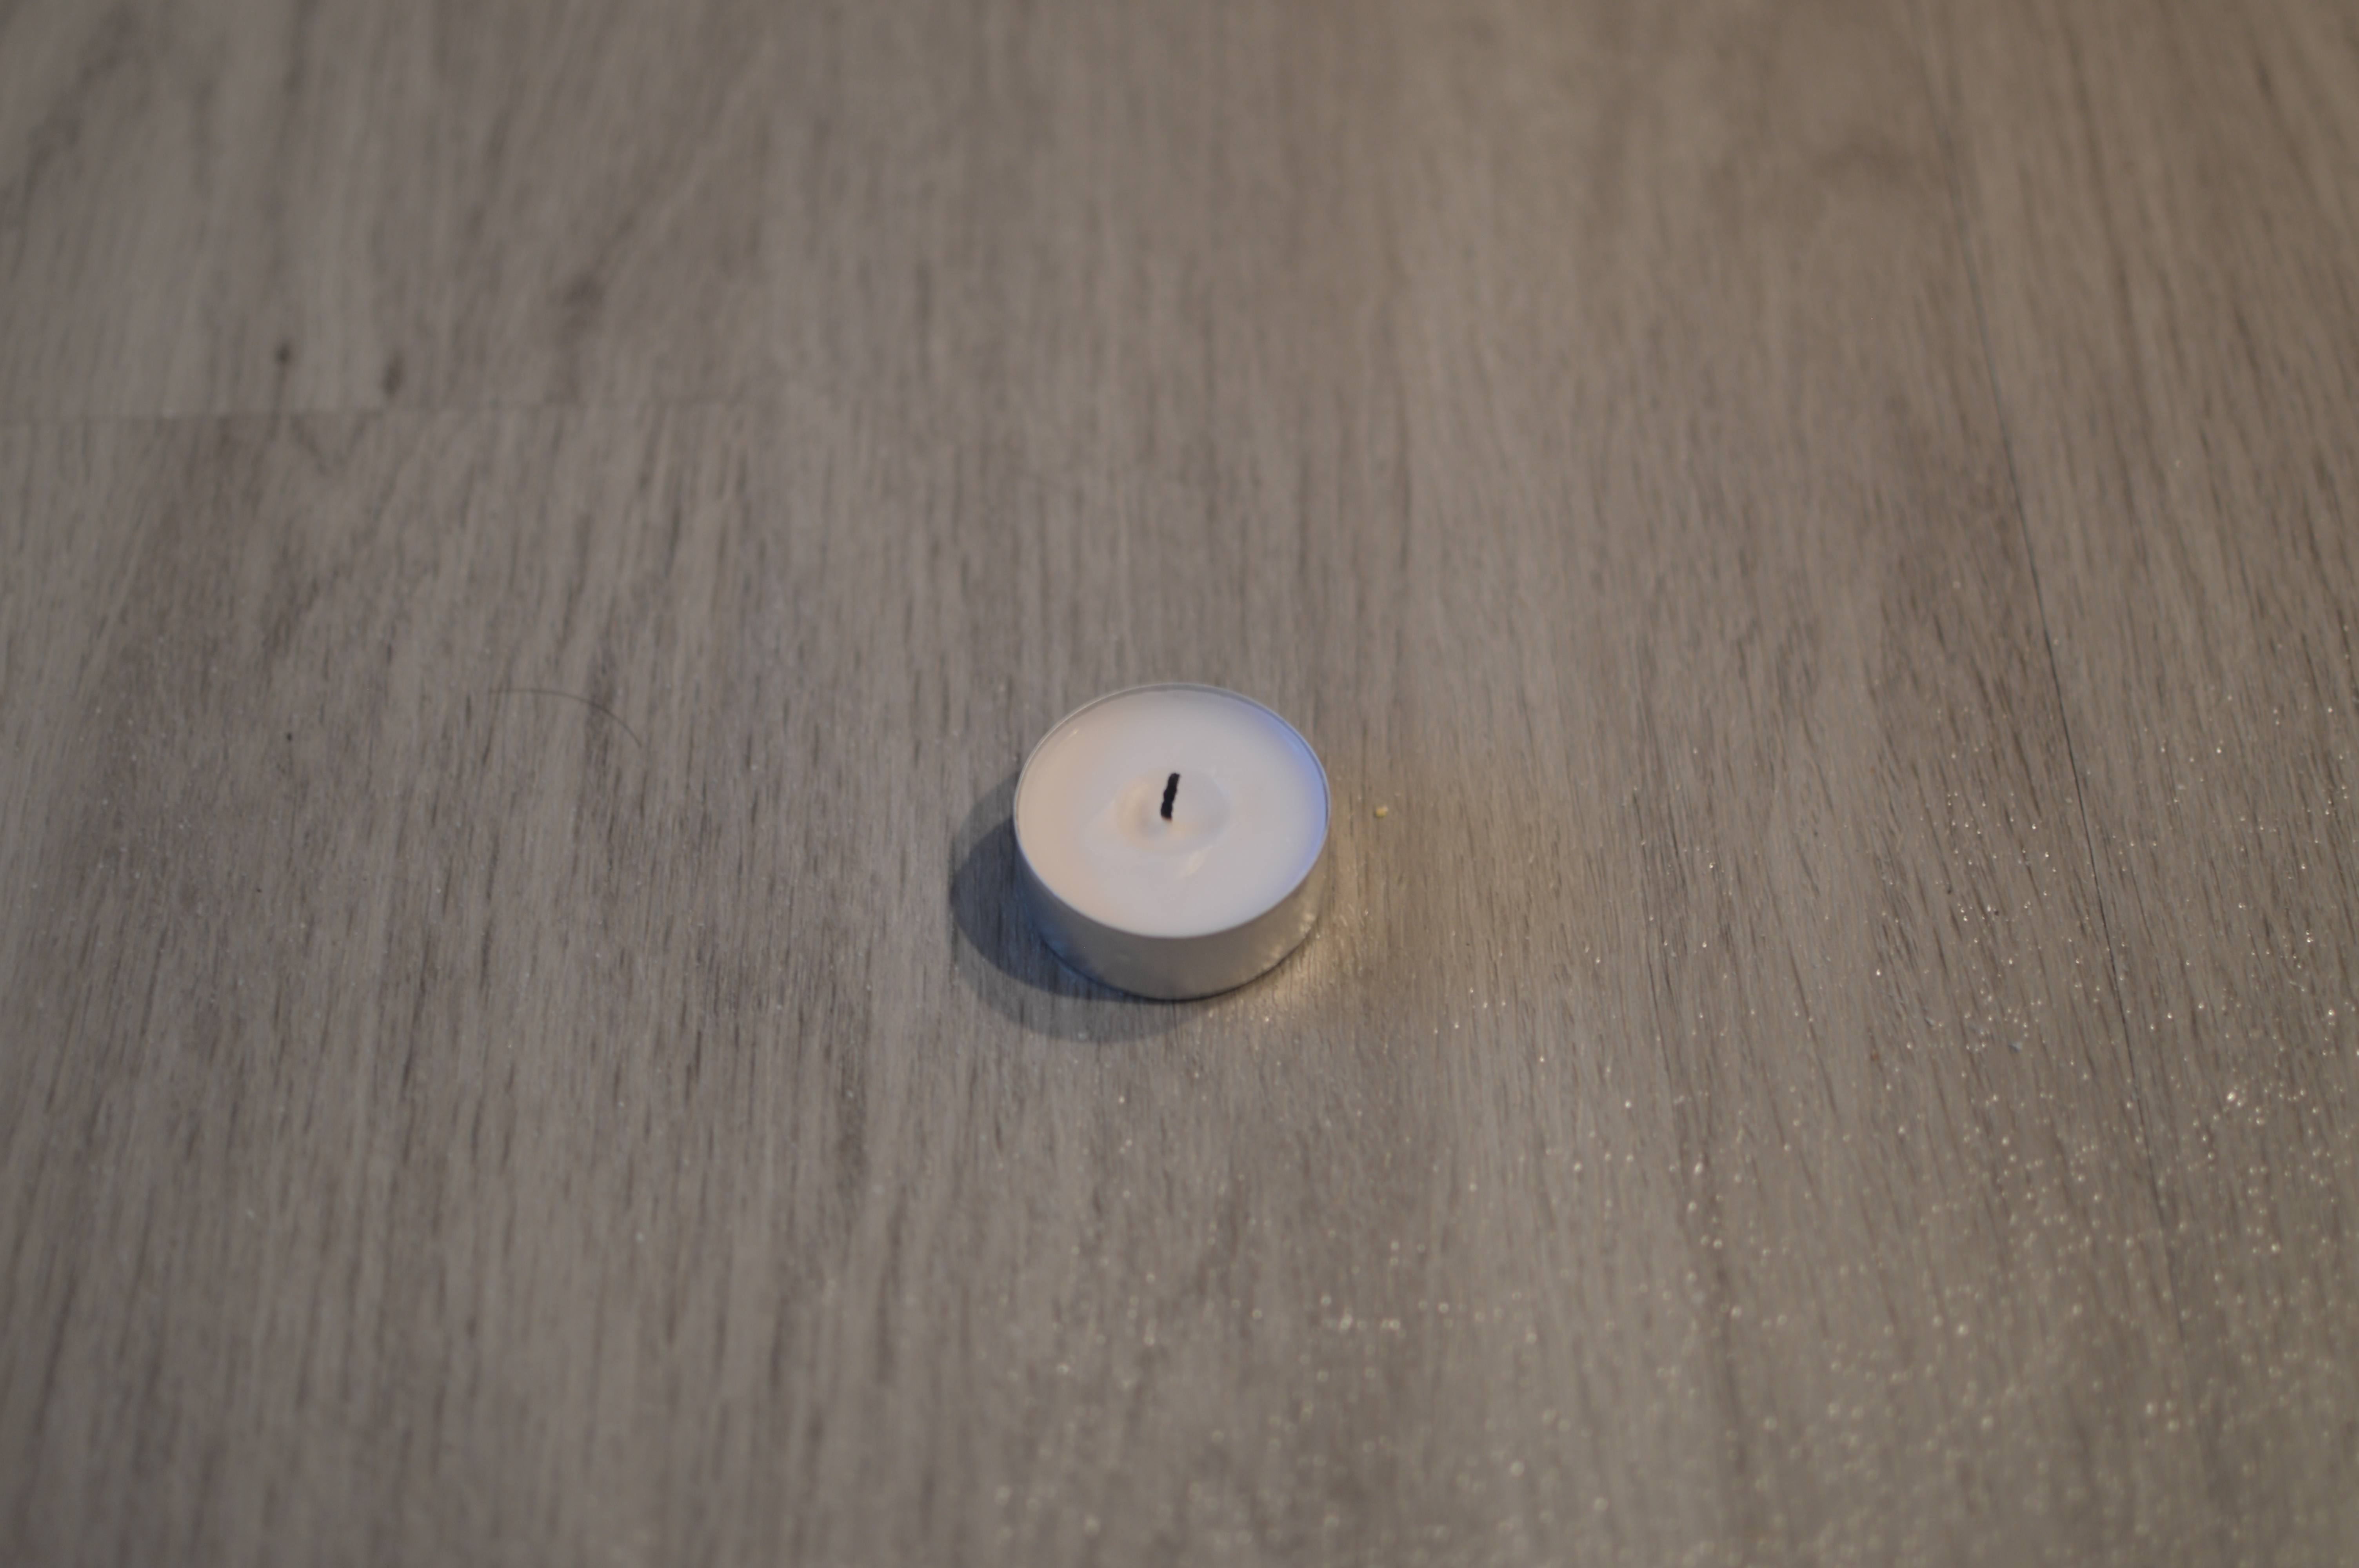
\includegraphics[width=0.95\textwidth]{Candle.JPG}
        \caption{}
        \label{fig:Candle}
    \end{subfigure}
    \begin{subfigure}[b]{0.23\textwidth}
    	\centering
        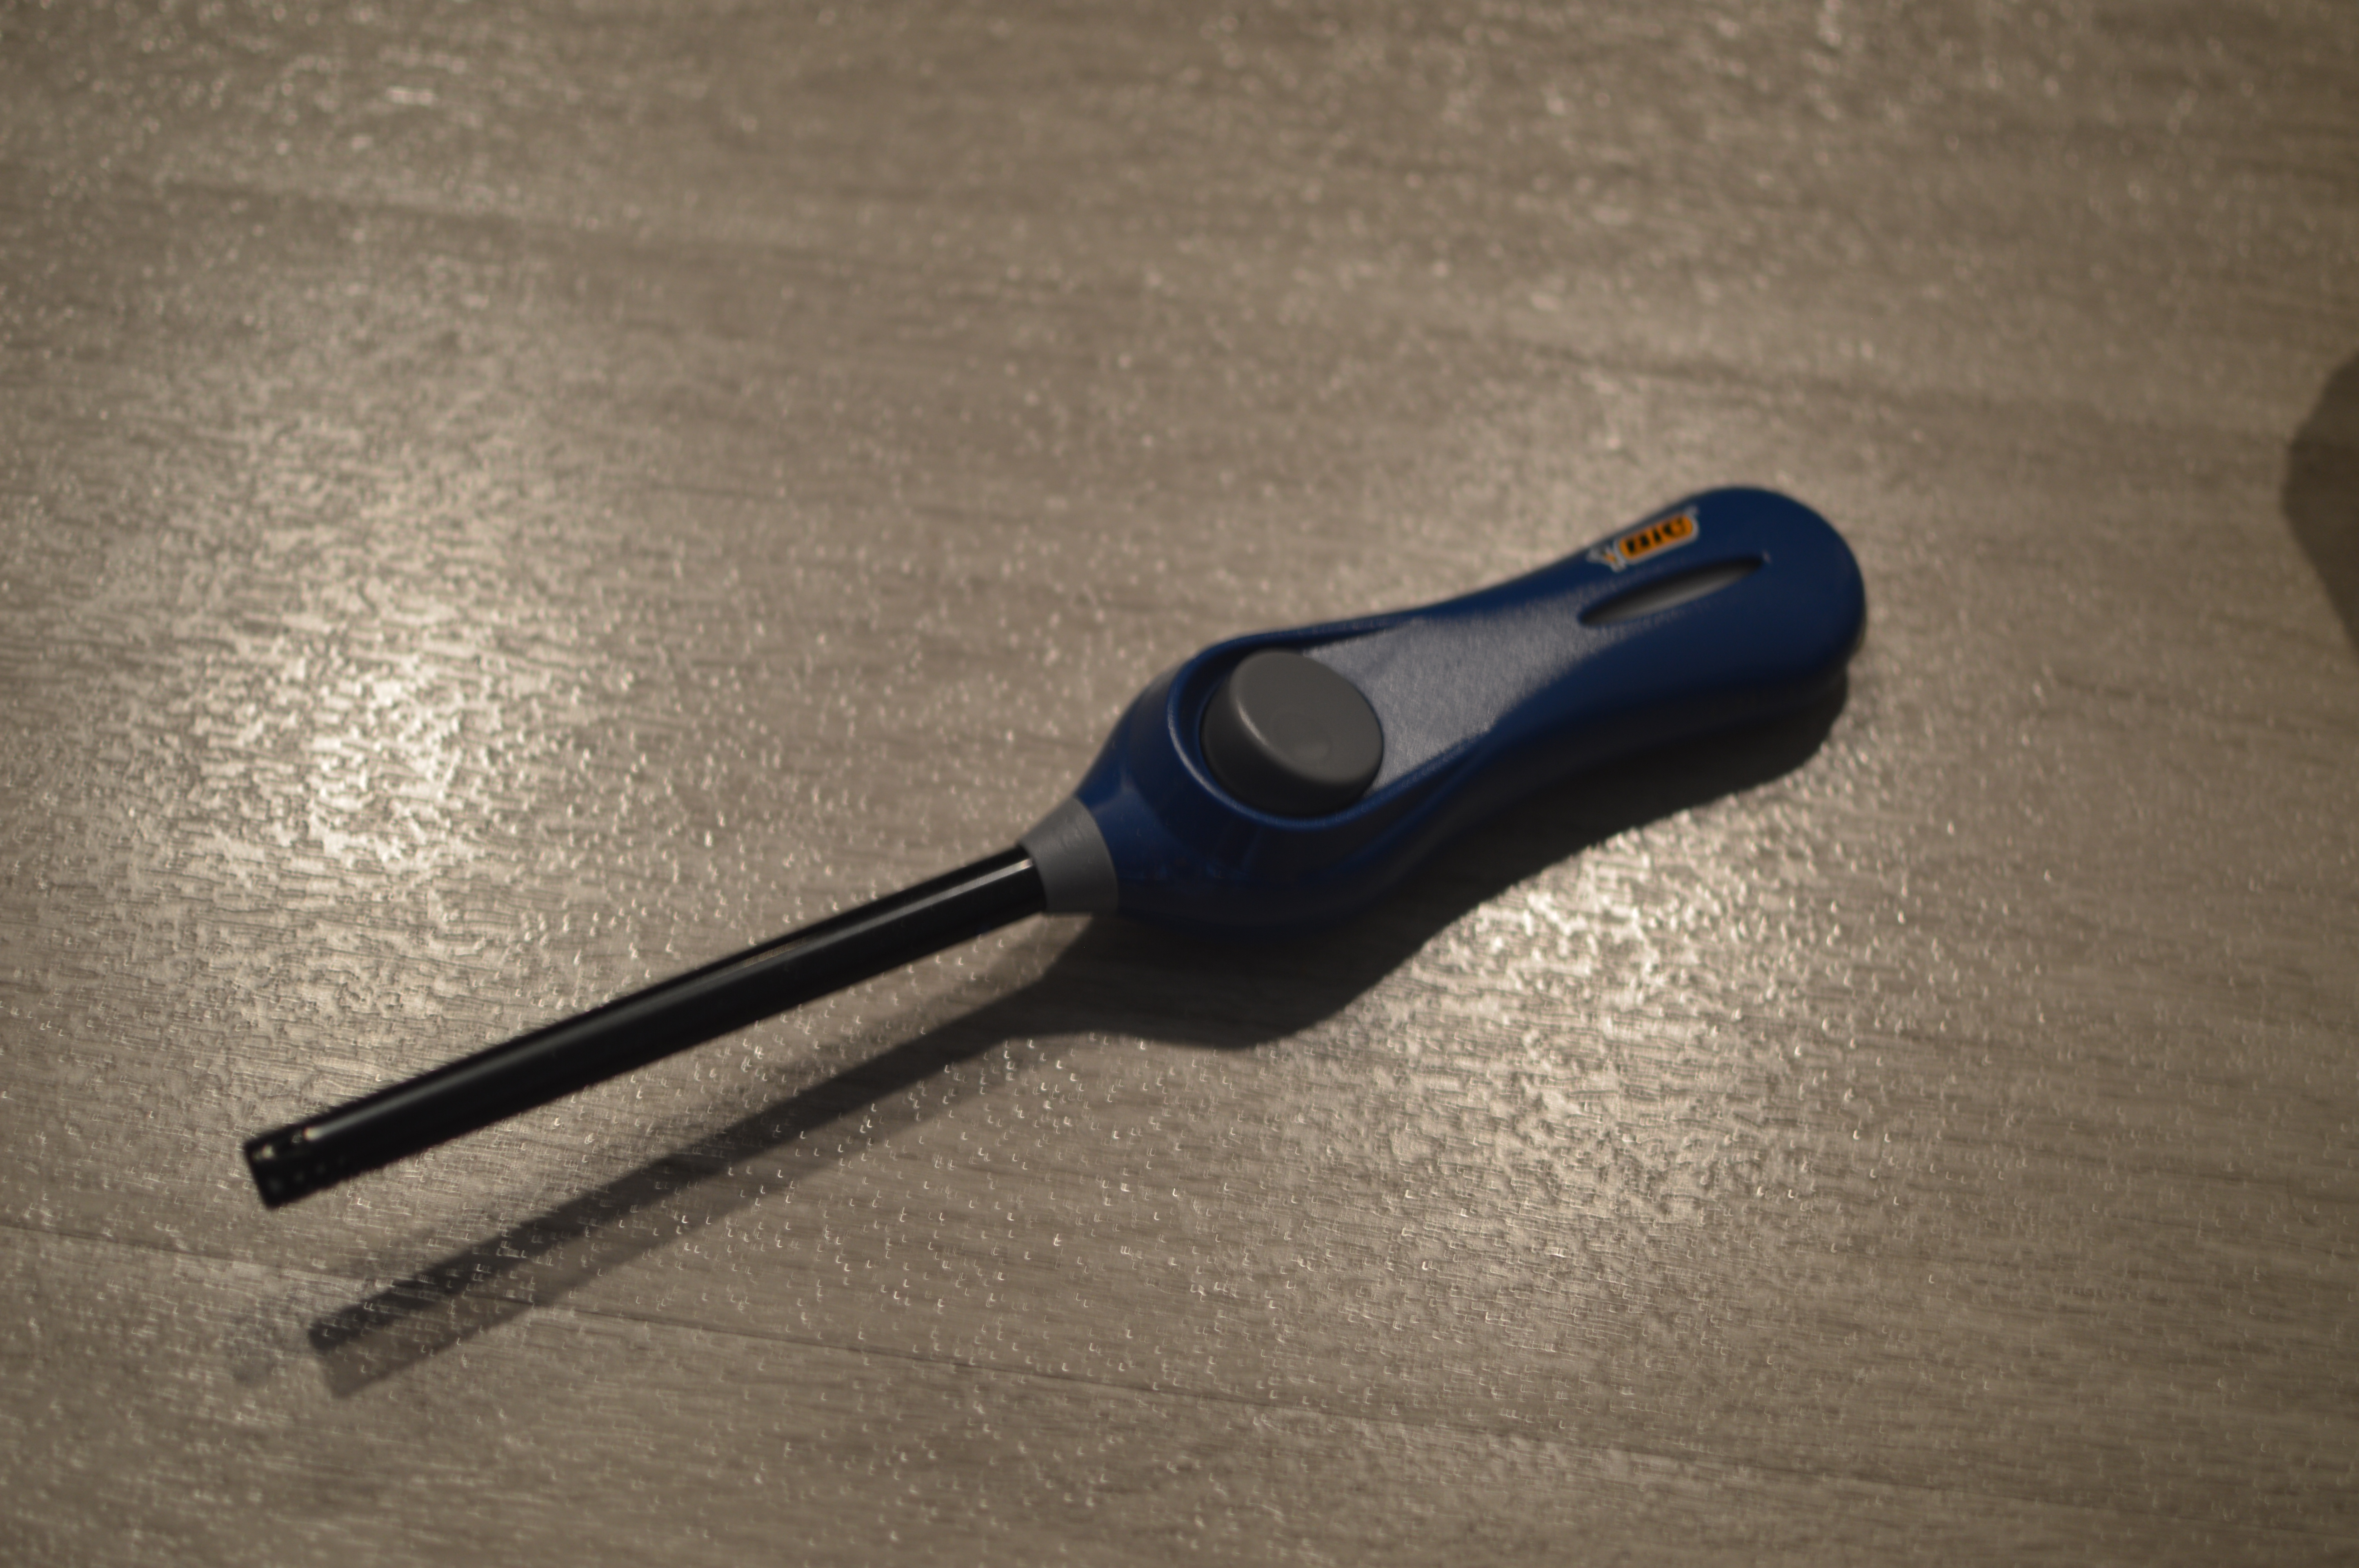
\includegraphics[width=0.95\textwidth]{Lighter.JPG}
        \caption{}
        \label{fig:Lighter}
    \end{subfigure}
    \begin{subfigure}[b]{0.23\textwidth}
    	\centering
        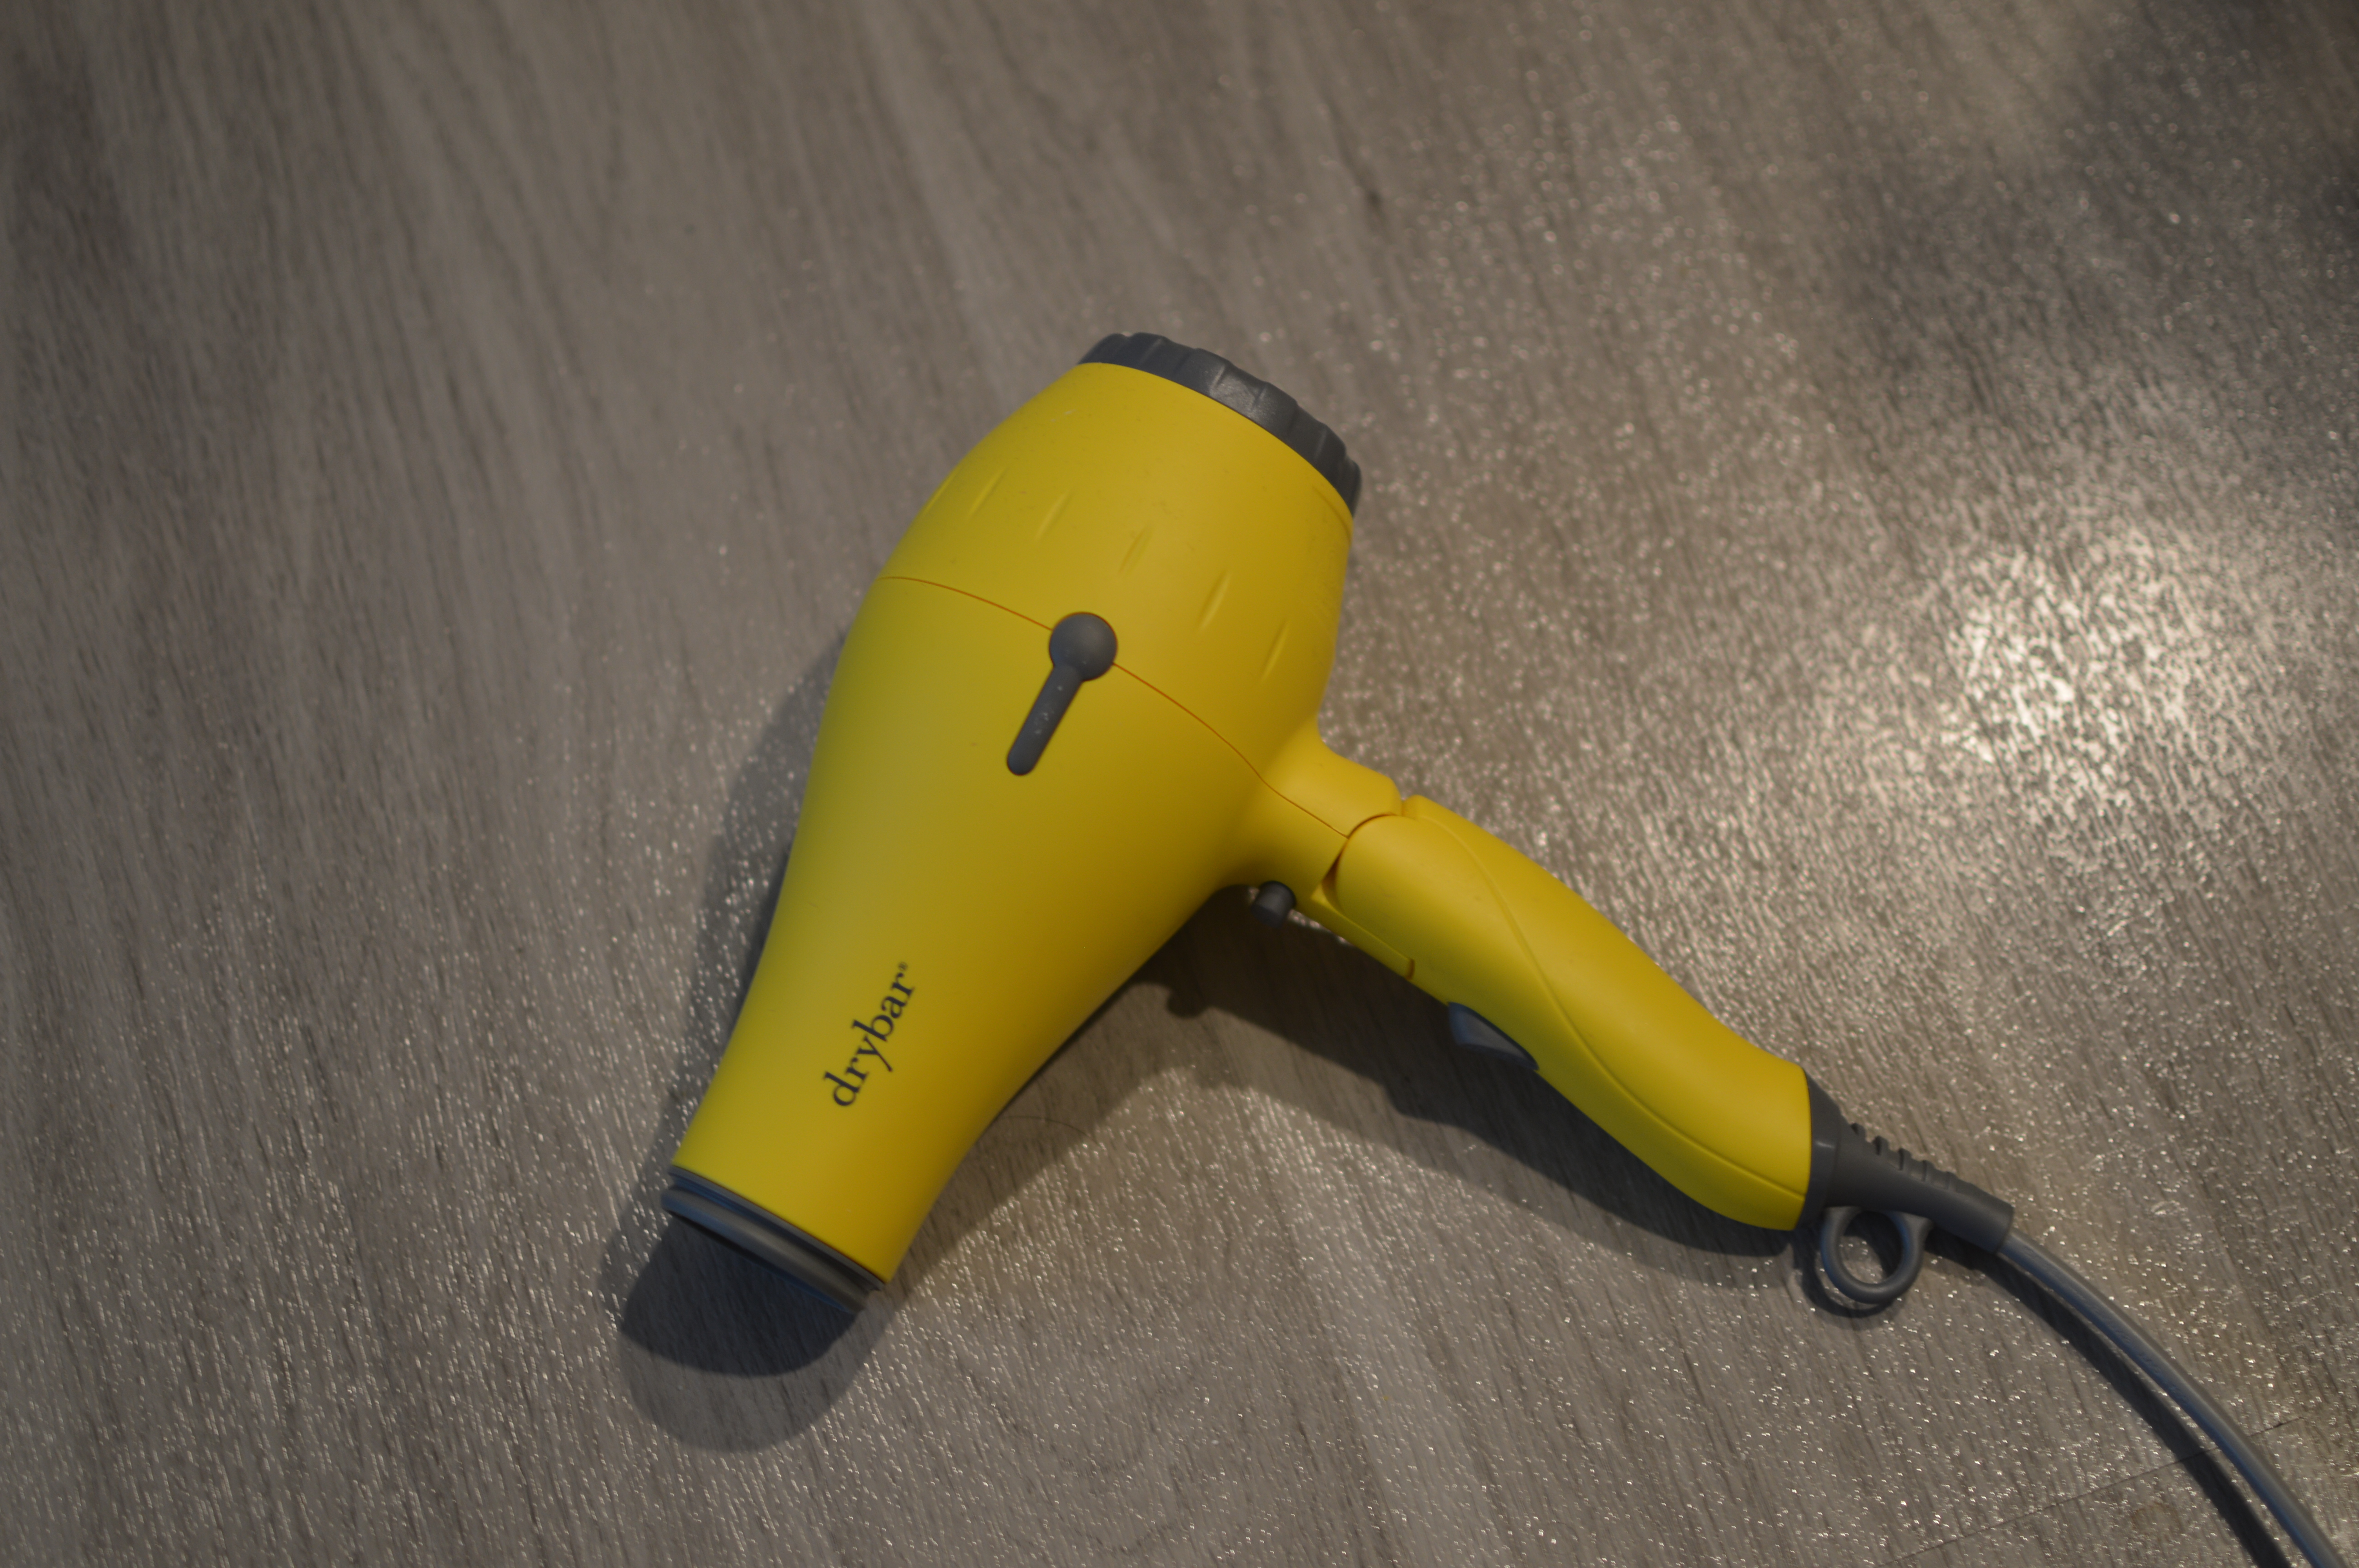
\includegraphics[width=0.95\textwidth]{Blow_Dryer.JPG}
        \caption{}
        \label{fig:Blow_Dryer}
    \end{subfigure}
    \begin{subfigure}[b]{0.23\textwidth}
    	\centering
        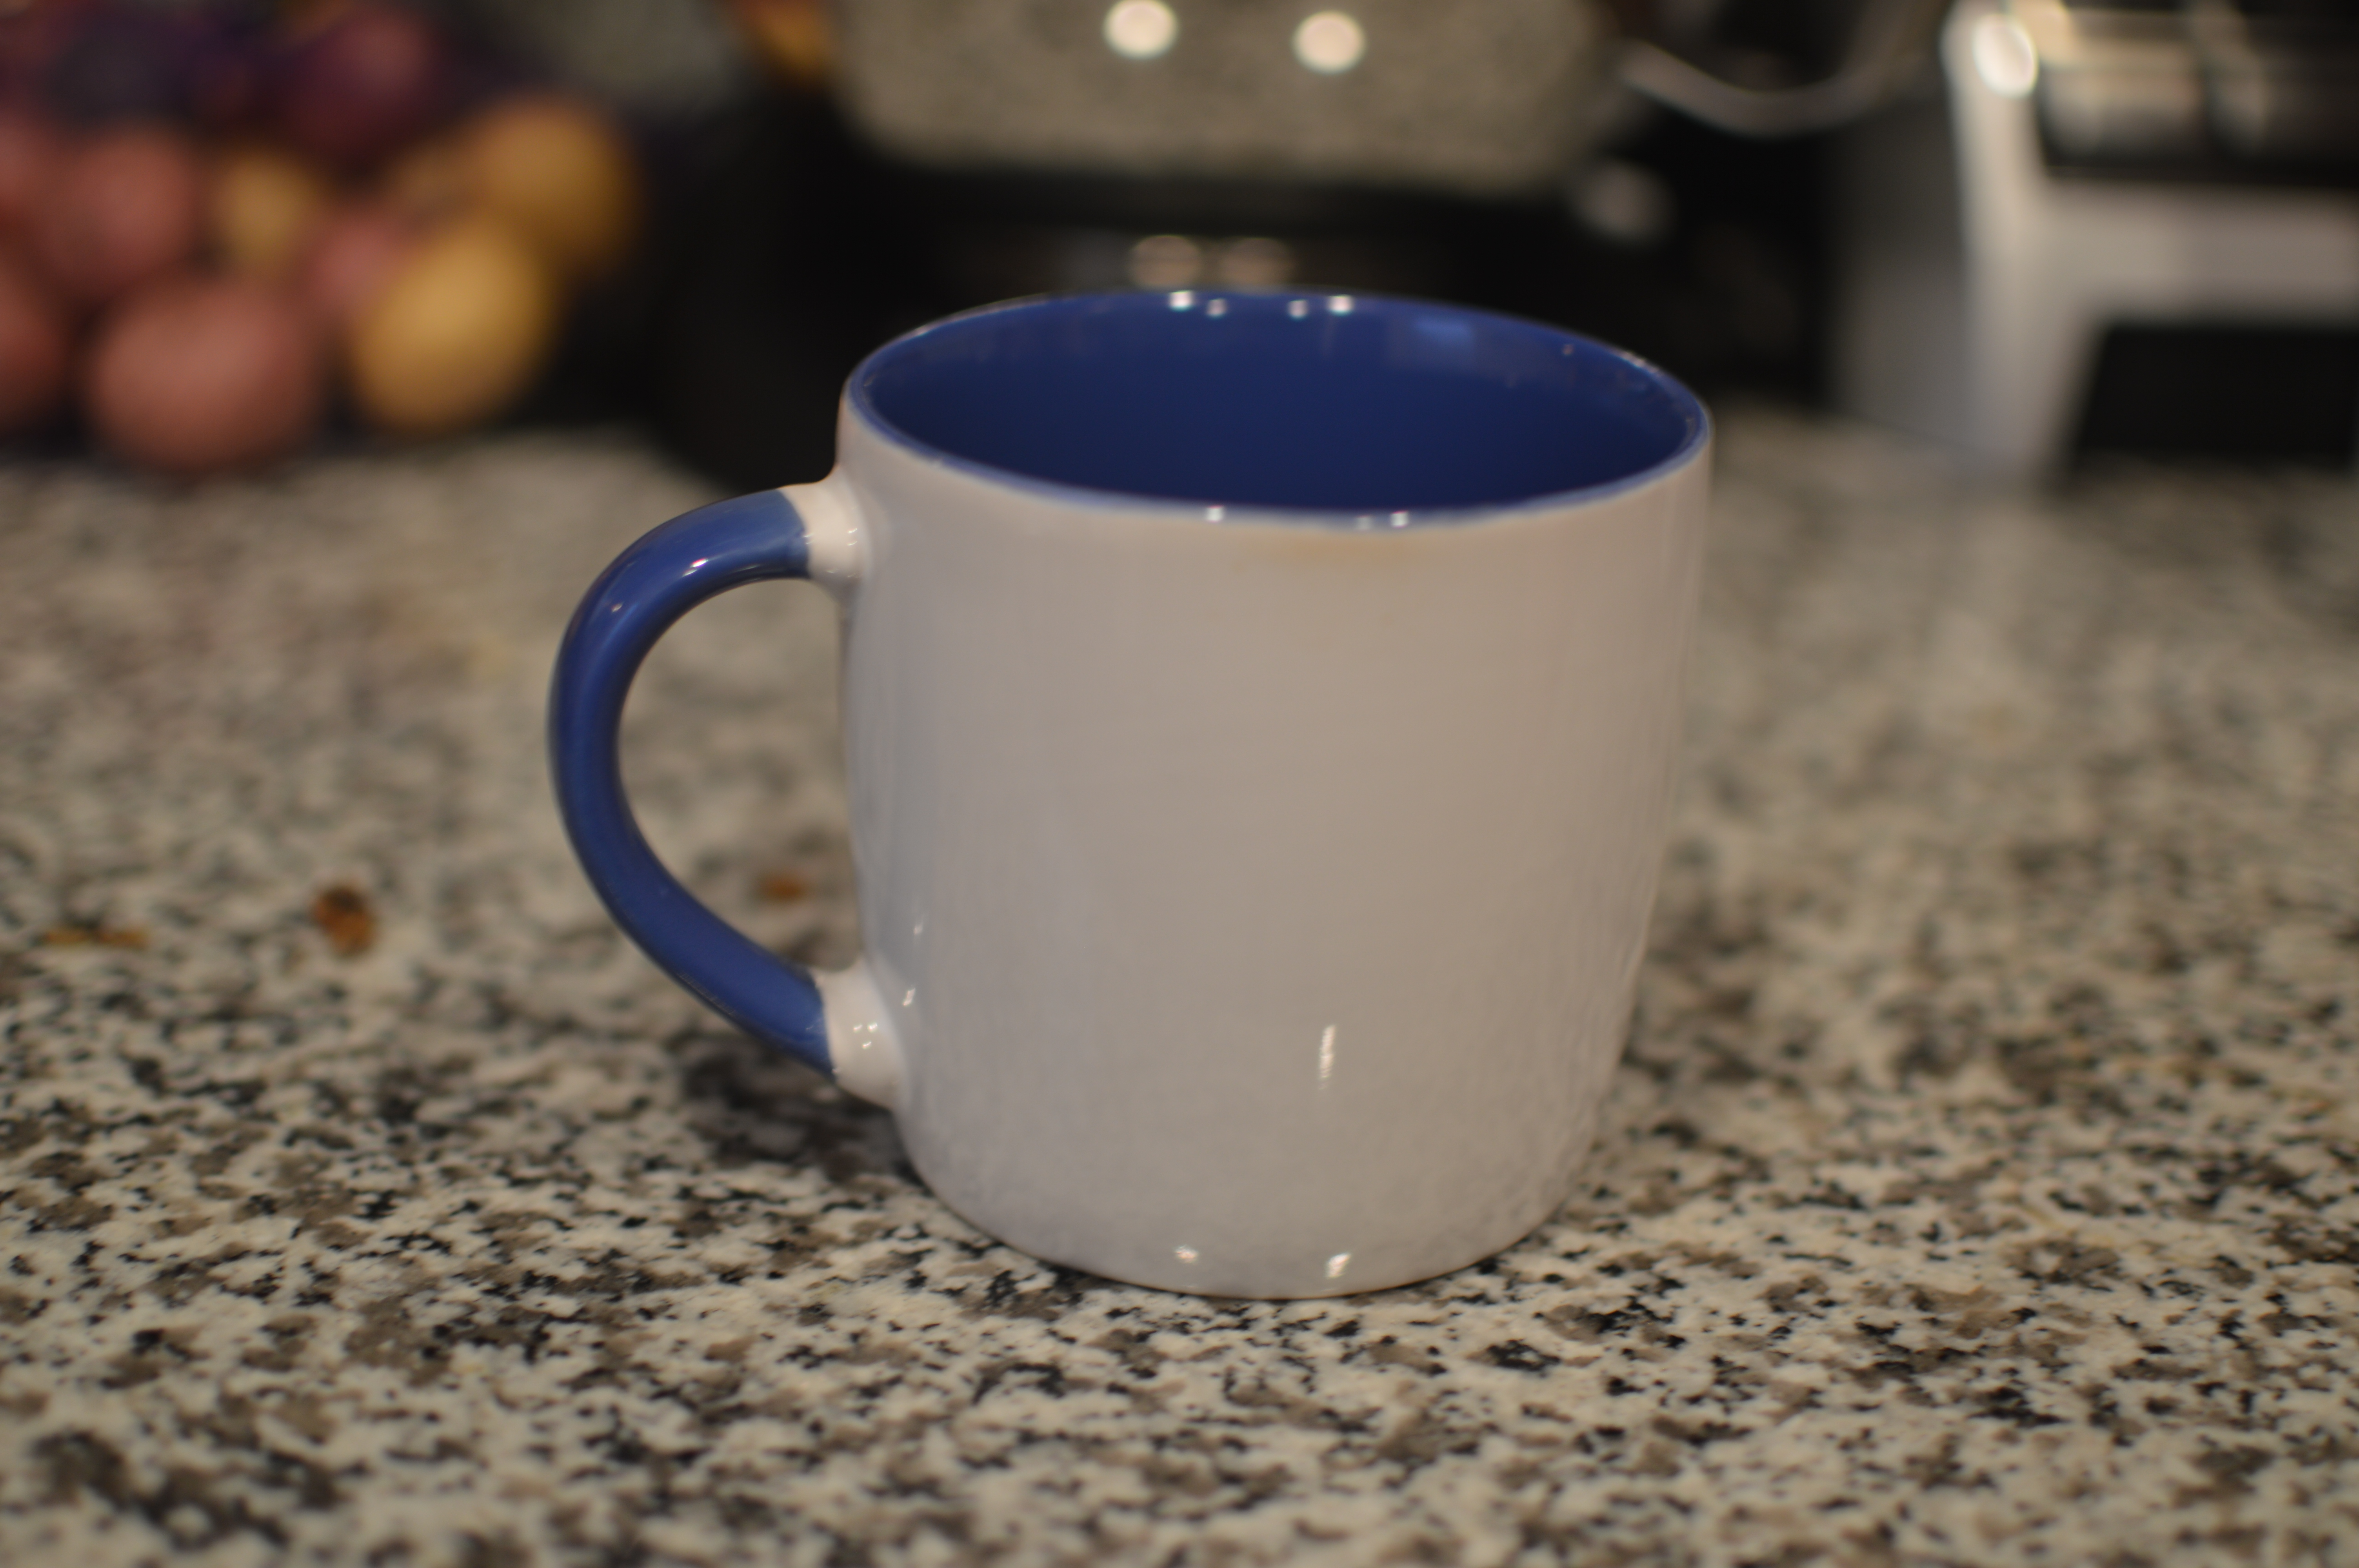
\includegraphics[width=0.95\textwidth]{Tea.JPG}
        \caption{}
        \label{fig:Tea}
    \end{subfigure}
    
    \caption{Objects used in the BOS experiments, including (a) a candle, (b) a lighter, (c) a blow dryer, and (d) a cup of tea.}
    \label{fig:Objects}
\end{figure}

The objects used are a candle, a lighter, a blow dryer, and a cup of tea.  These are pretty straight-forward.  The candle and lighter provide the biggest temperature (and thus density and index of refraction) gradient, and are easily used as a benchmark test case for different backgrounds.  If you can't see the signal from these two, you're already in trouble.  The blow dryer also gets quite hot, but provides a more turbulent flow that that close to the candle or lighter flame.  The tea tests the ability to see weaker gradients.

% FIGURE: Backgrounds
\begin{figure}[h]
    \centering
    \begin{subfigure}[b]{0.23\textwidth}
    	\centering
        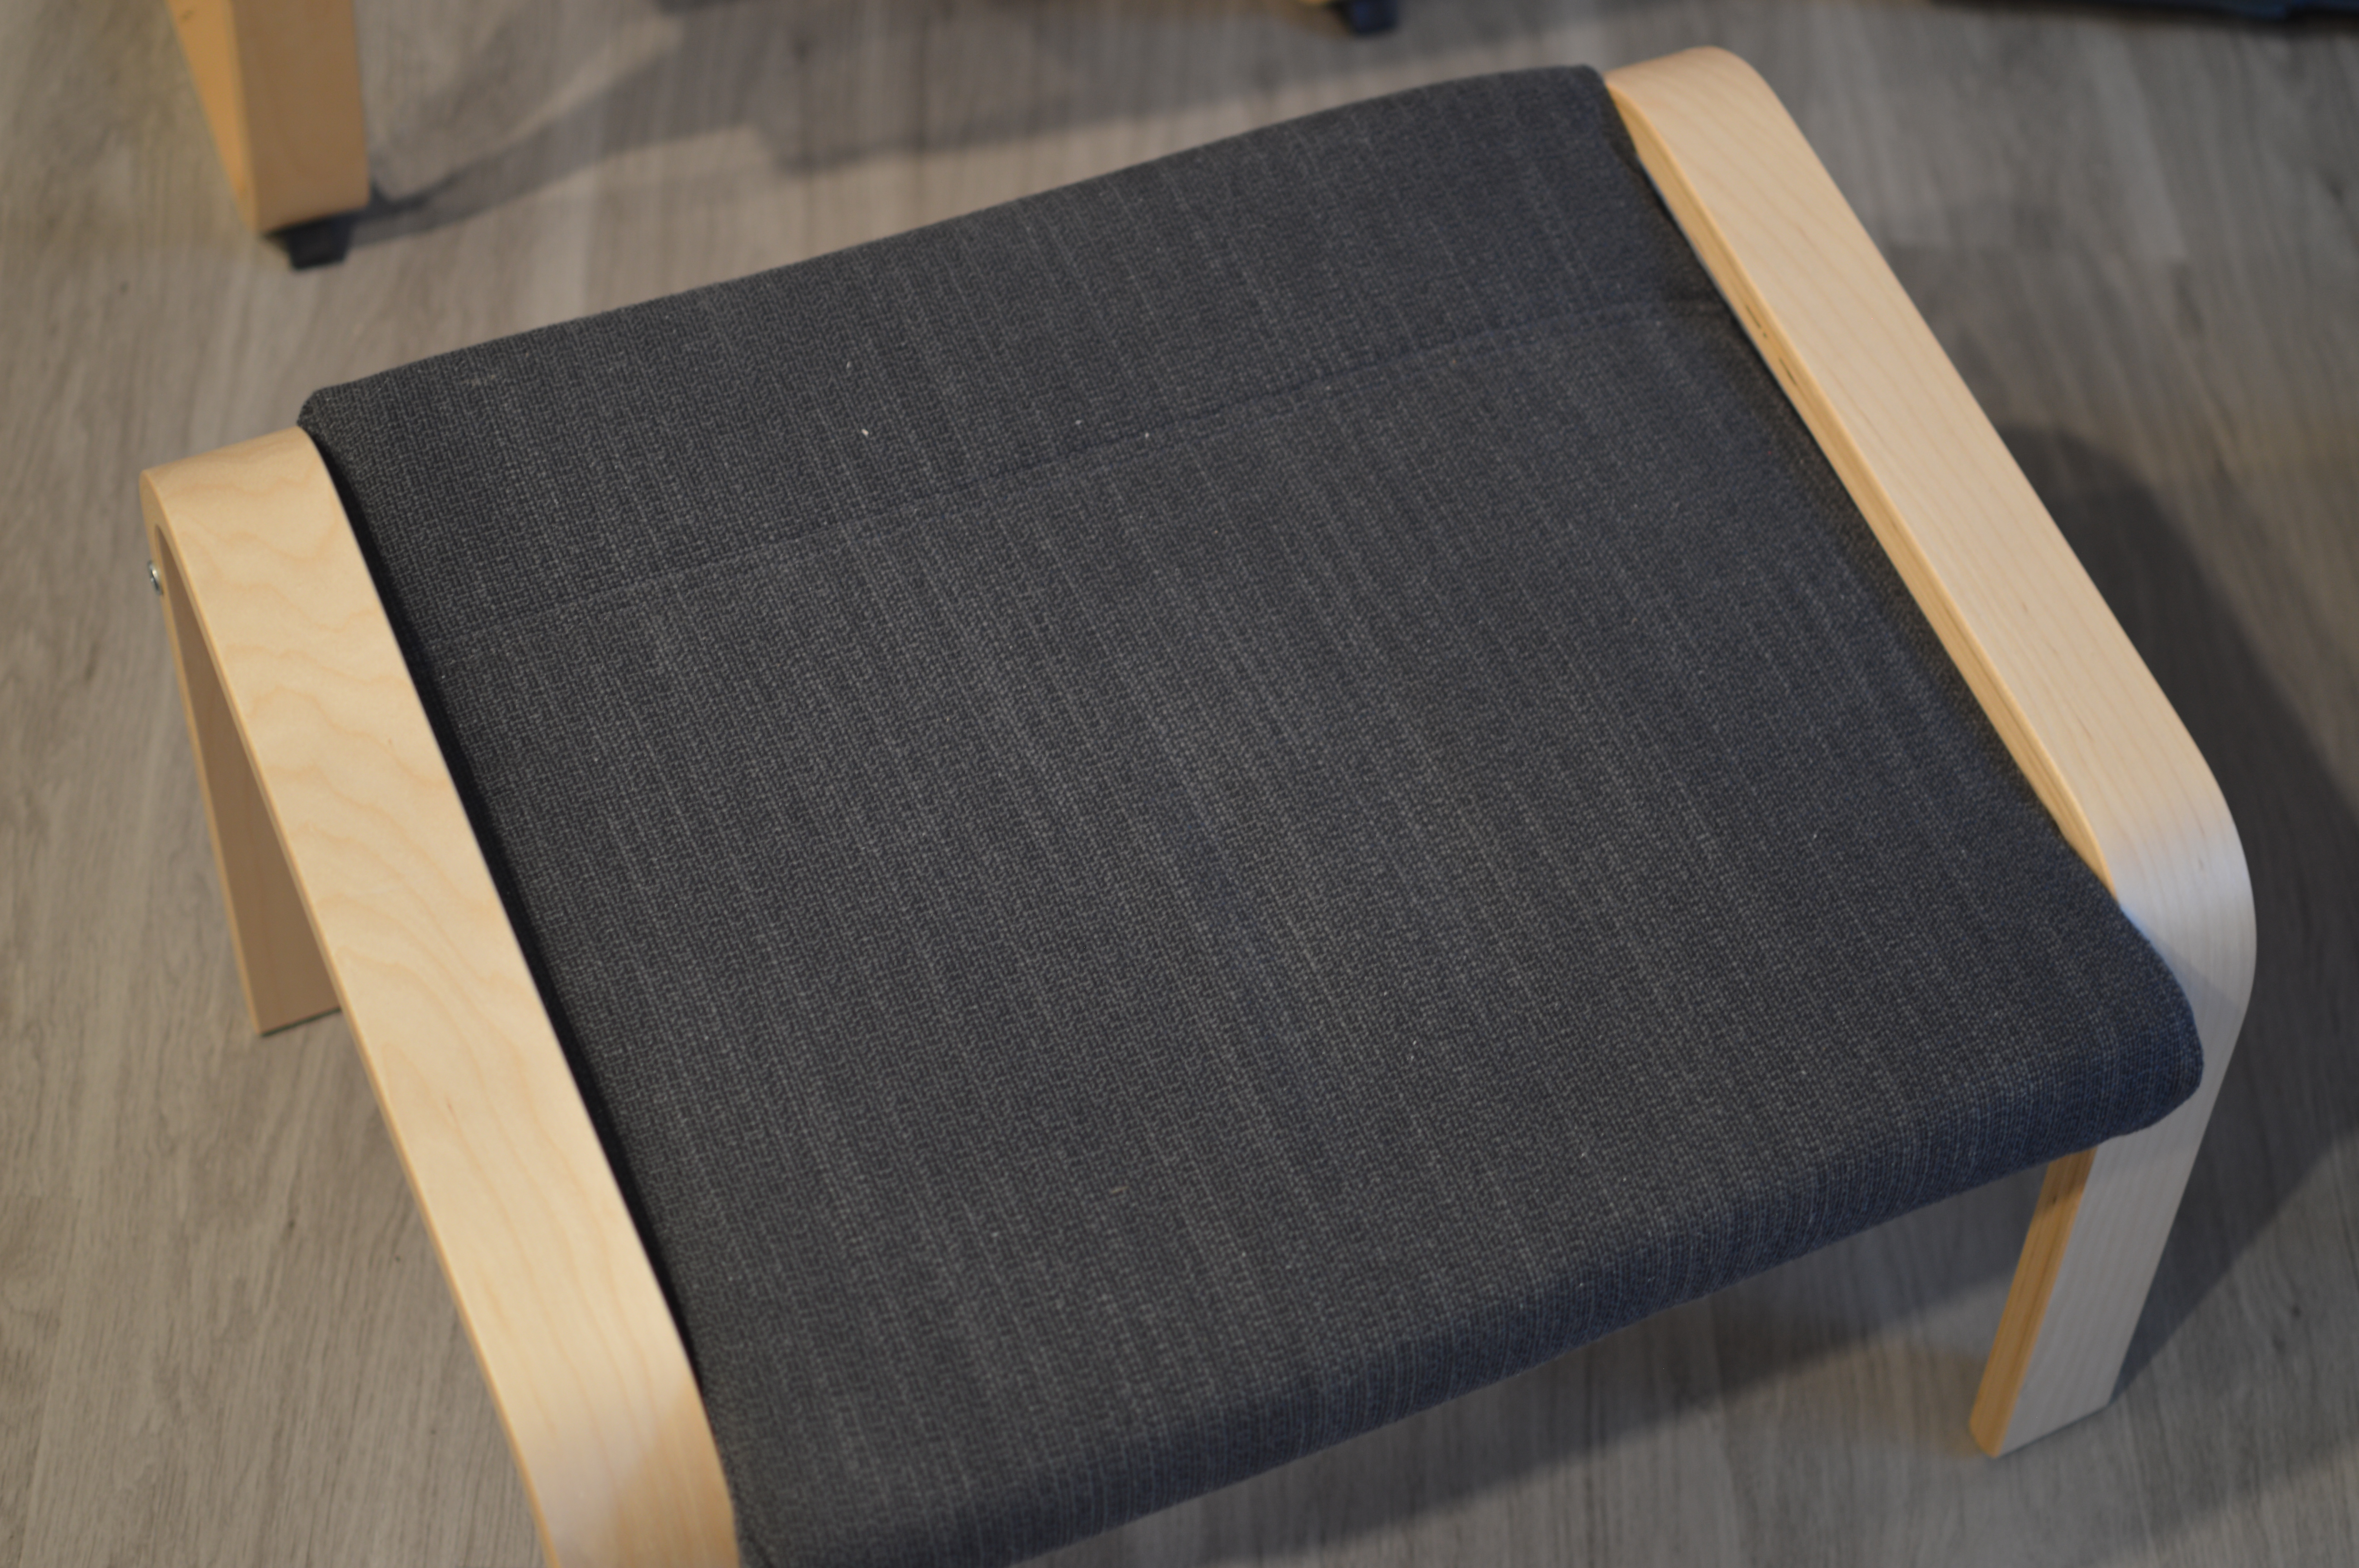
\includegraphics[width=0.95\textwidth]{IKEA_Chair.JPG}
        \caption{}
        \label{fig:IKEA_Chair}
    \end{subfigure}
    \begin{subfigure}[b]{0.23\textwidth}
    	\centering
        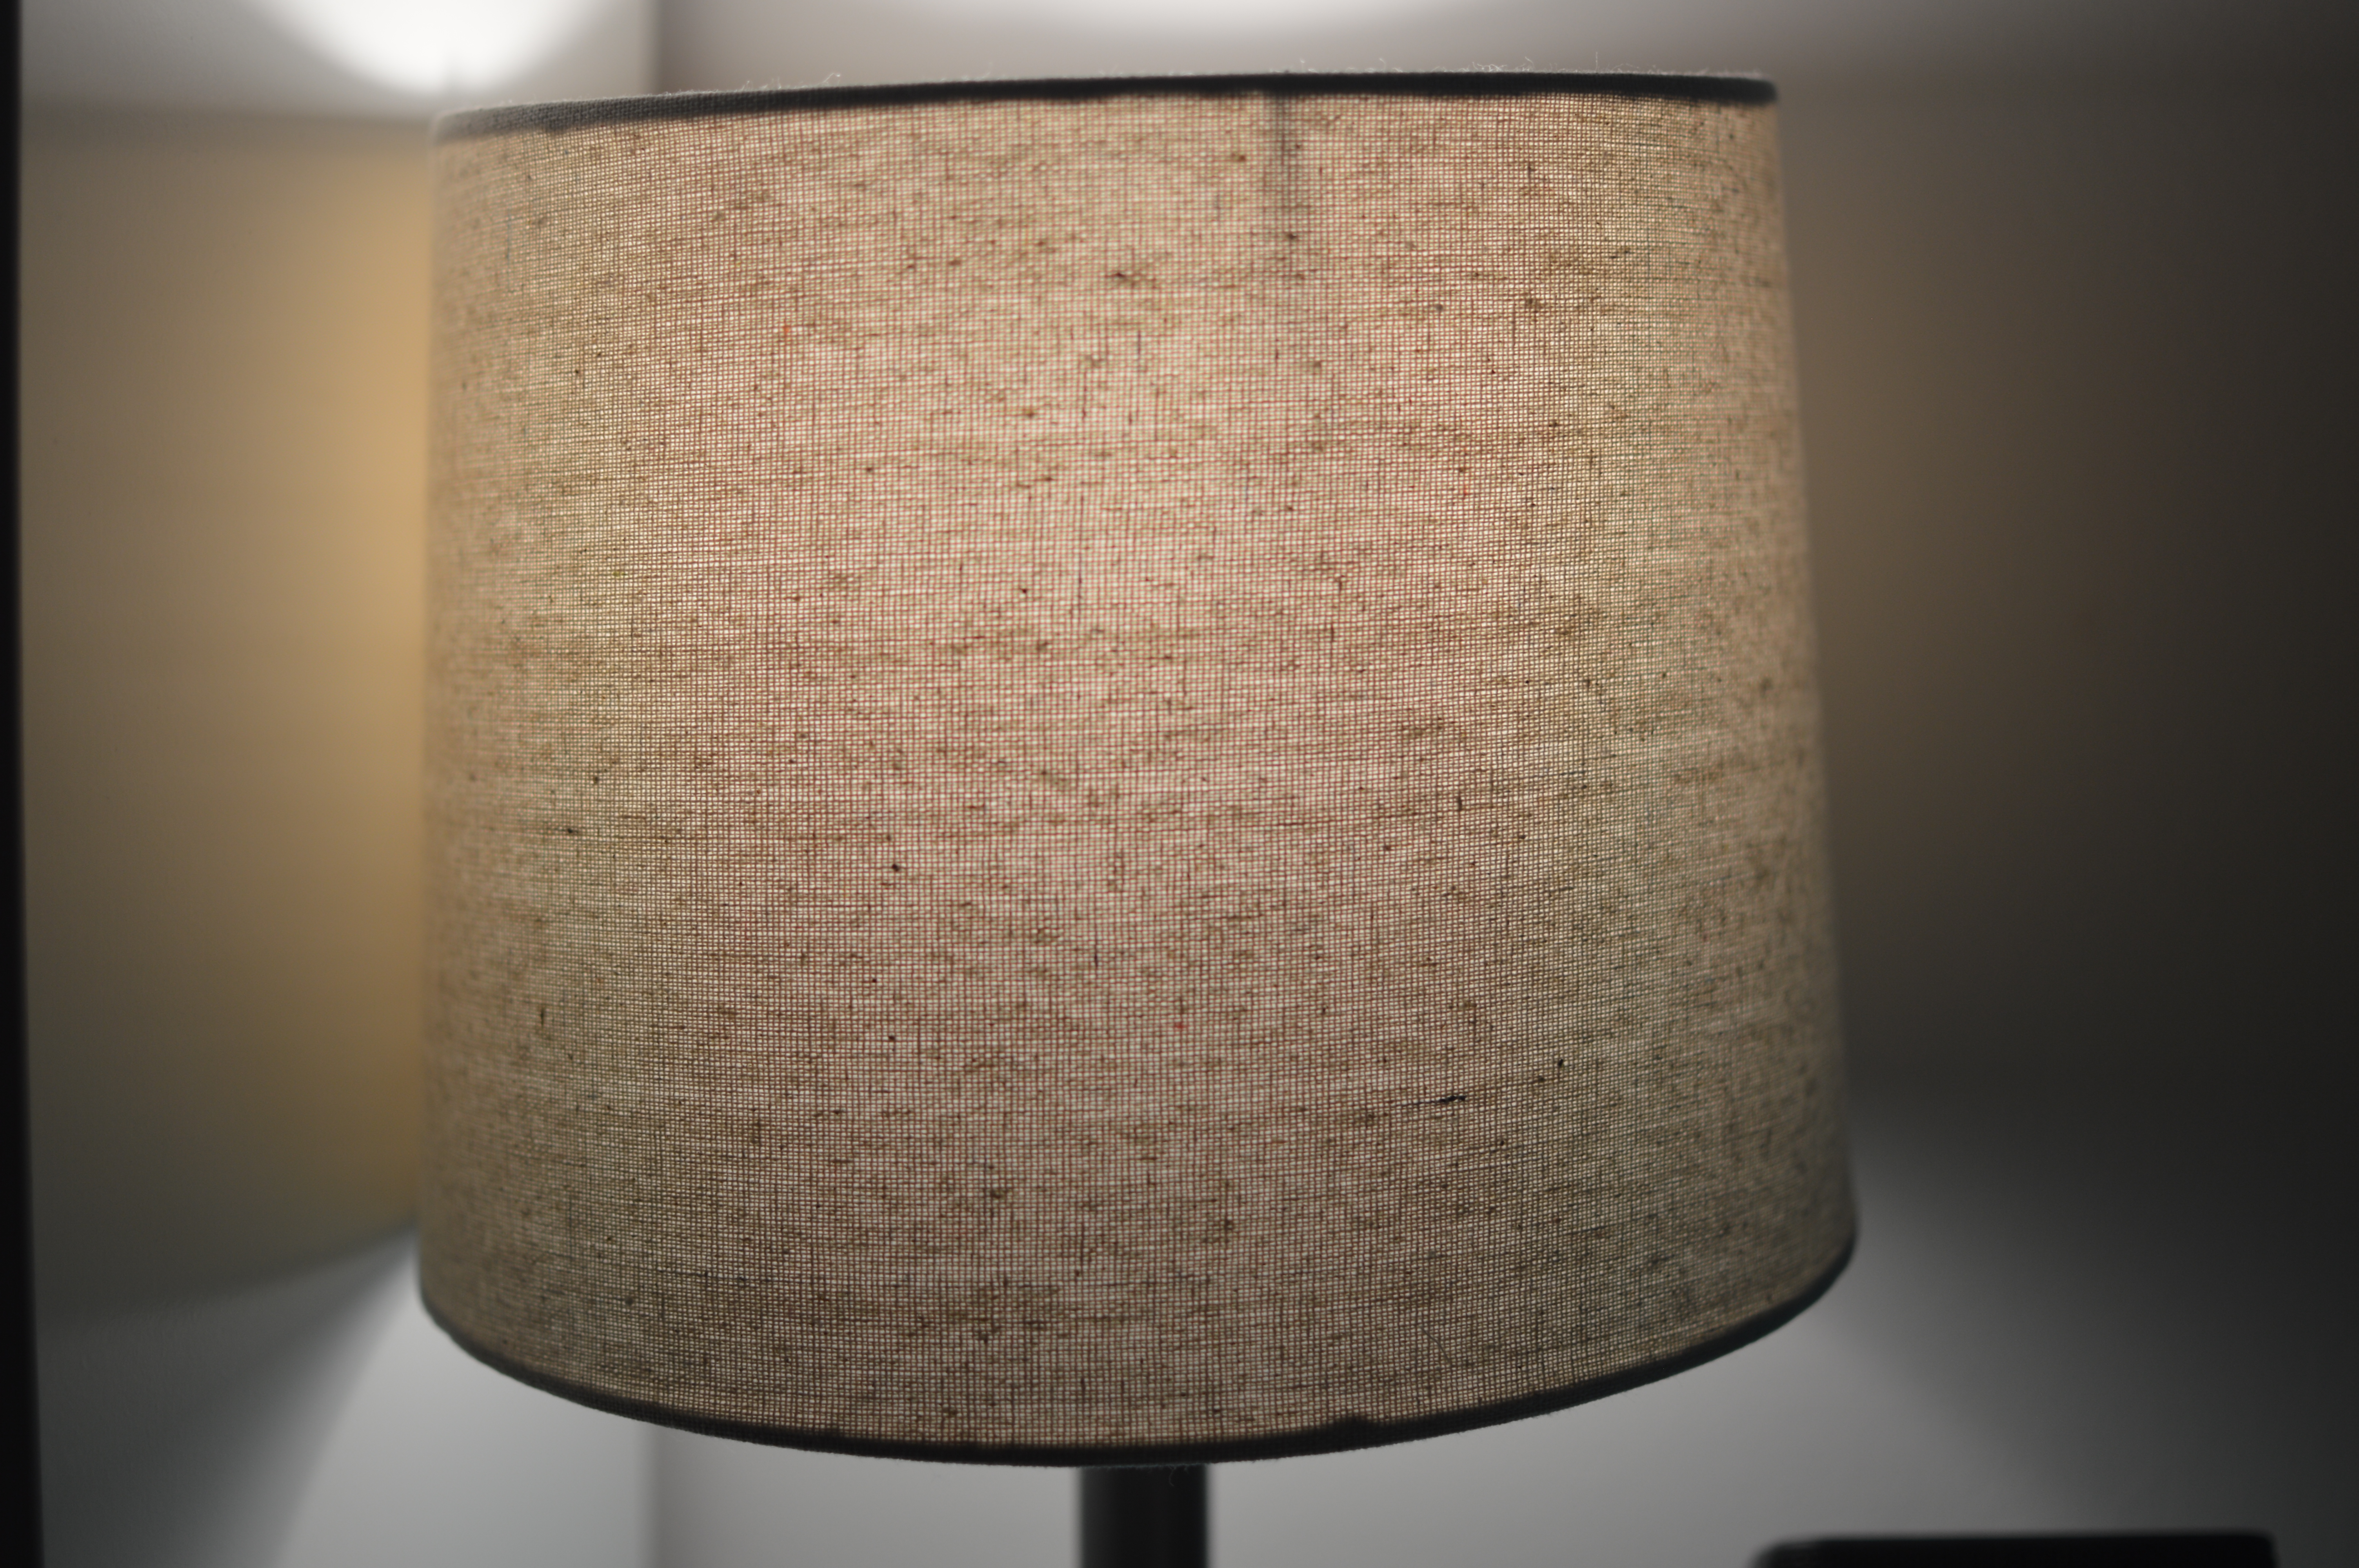
\includegraphics[width=0.95\textwidth]{Lamp_Shade.JPG}
        \caption{}
        \label{fig:Lamp_Shade}
    \end{subfigure}
    \begin{subfigure}[b]{0.23\textwidth}
    	\centering
        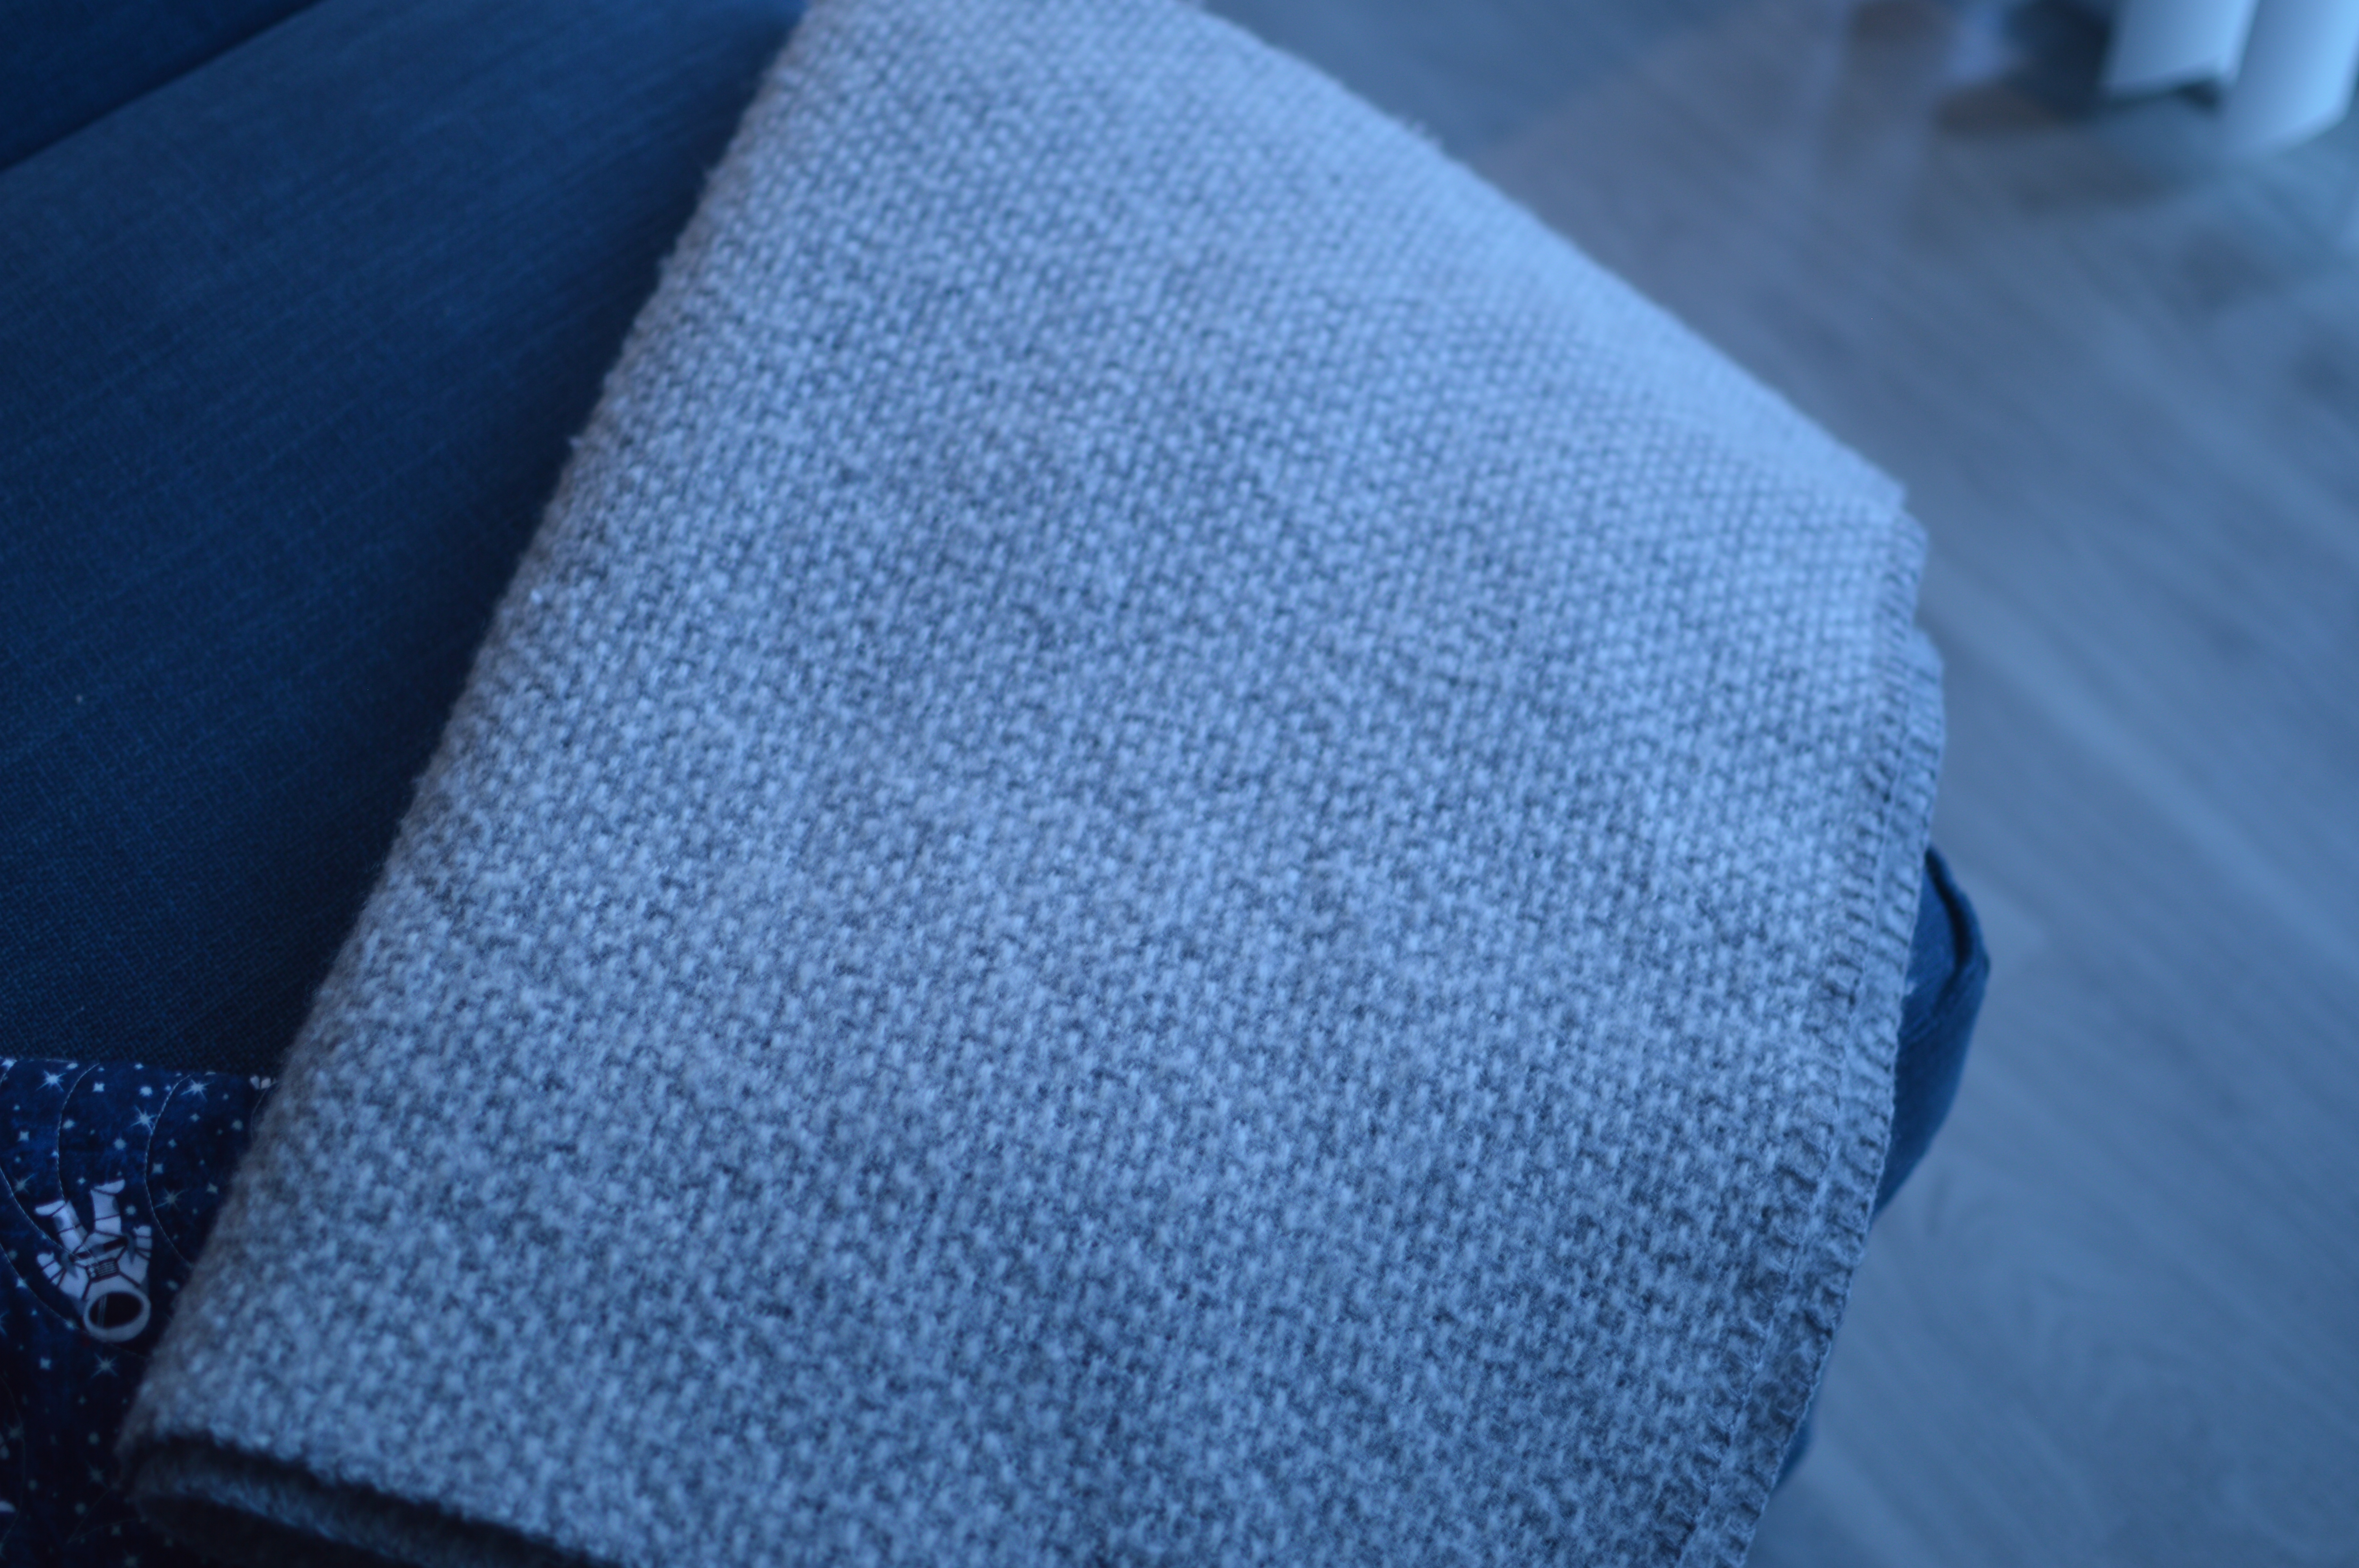
\includegraphics[width=0.95\textwidth]{Blanket.JPG}
        \caption{}
        \label{fig:Blanket}
    \end{subfigure}
    \begin{subfigure}[b]{0.23\textwidth}
    	\centering
        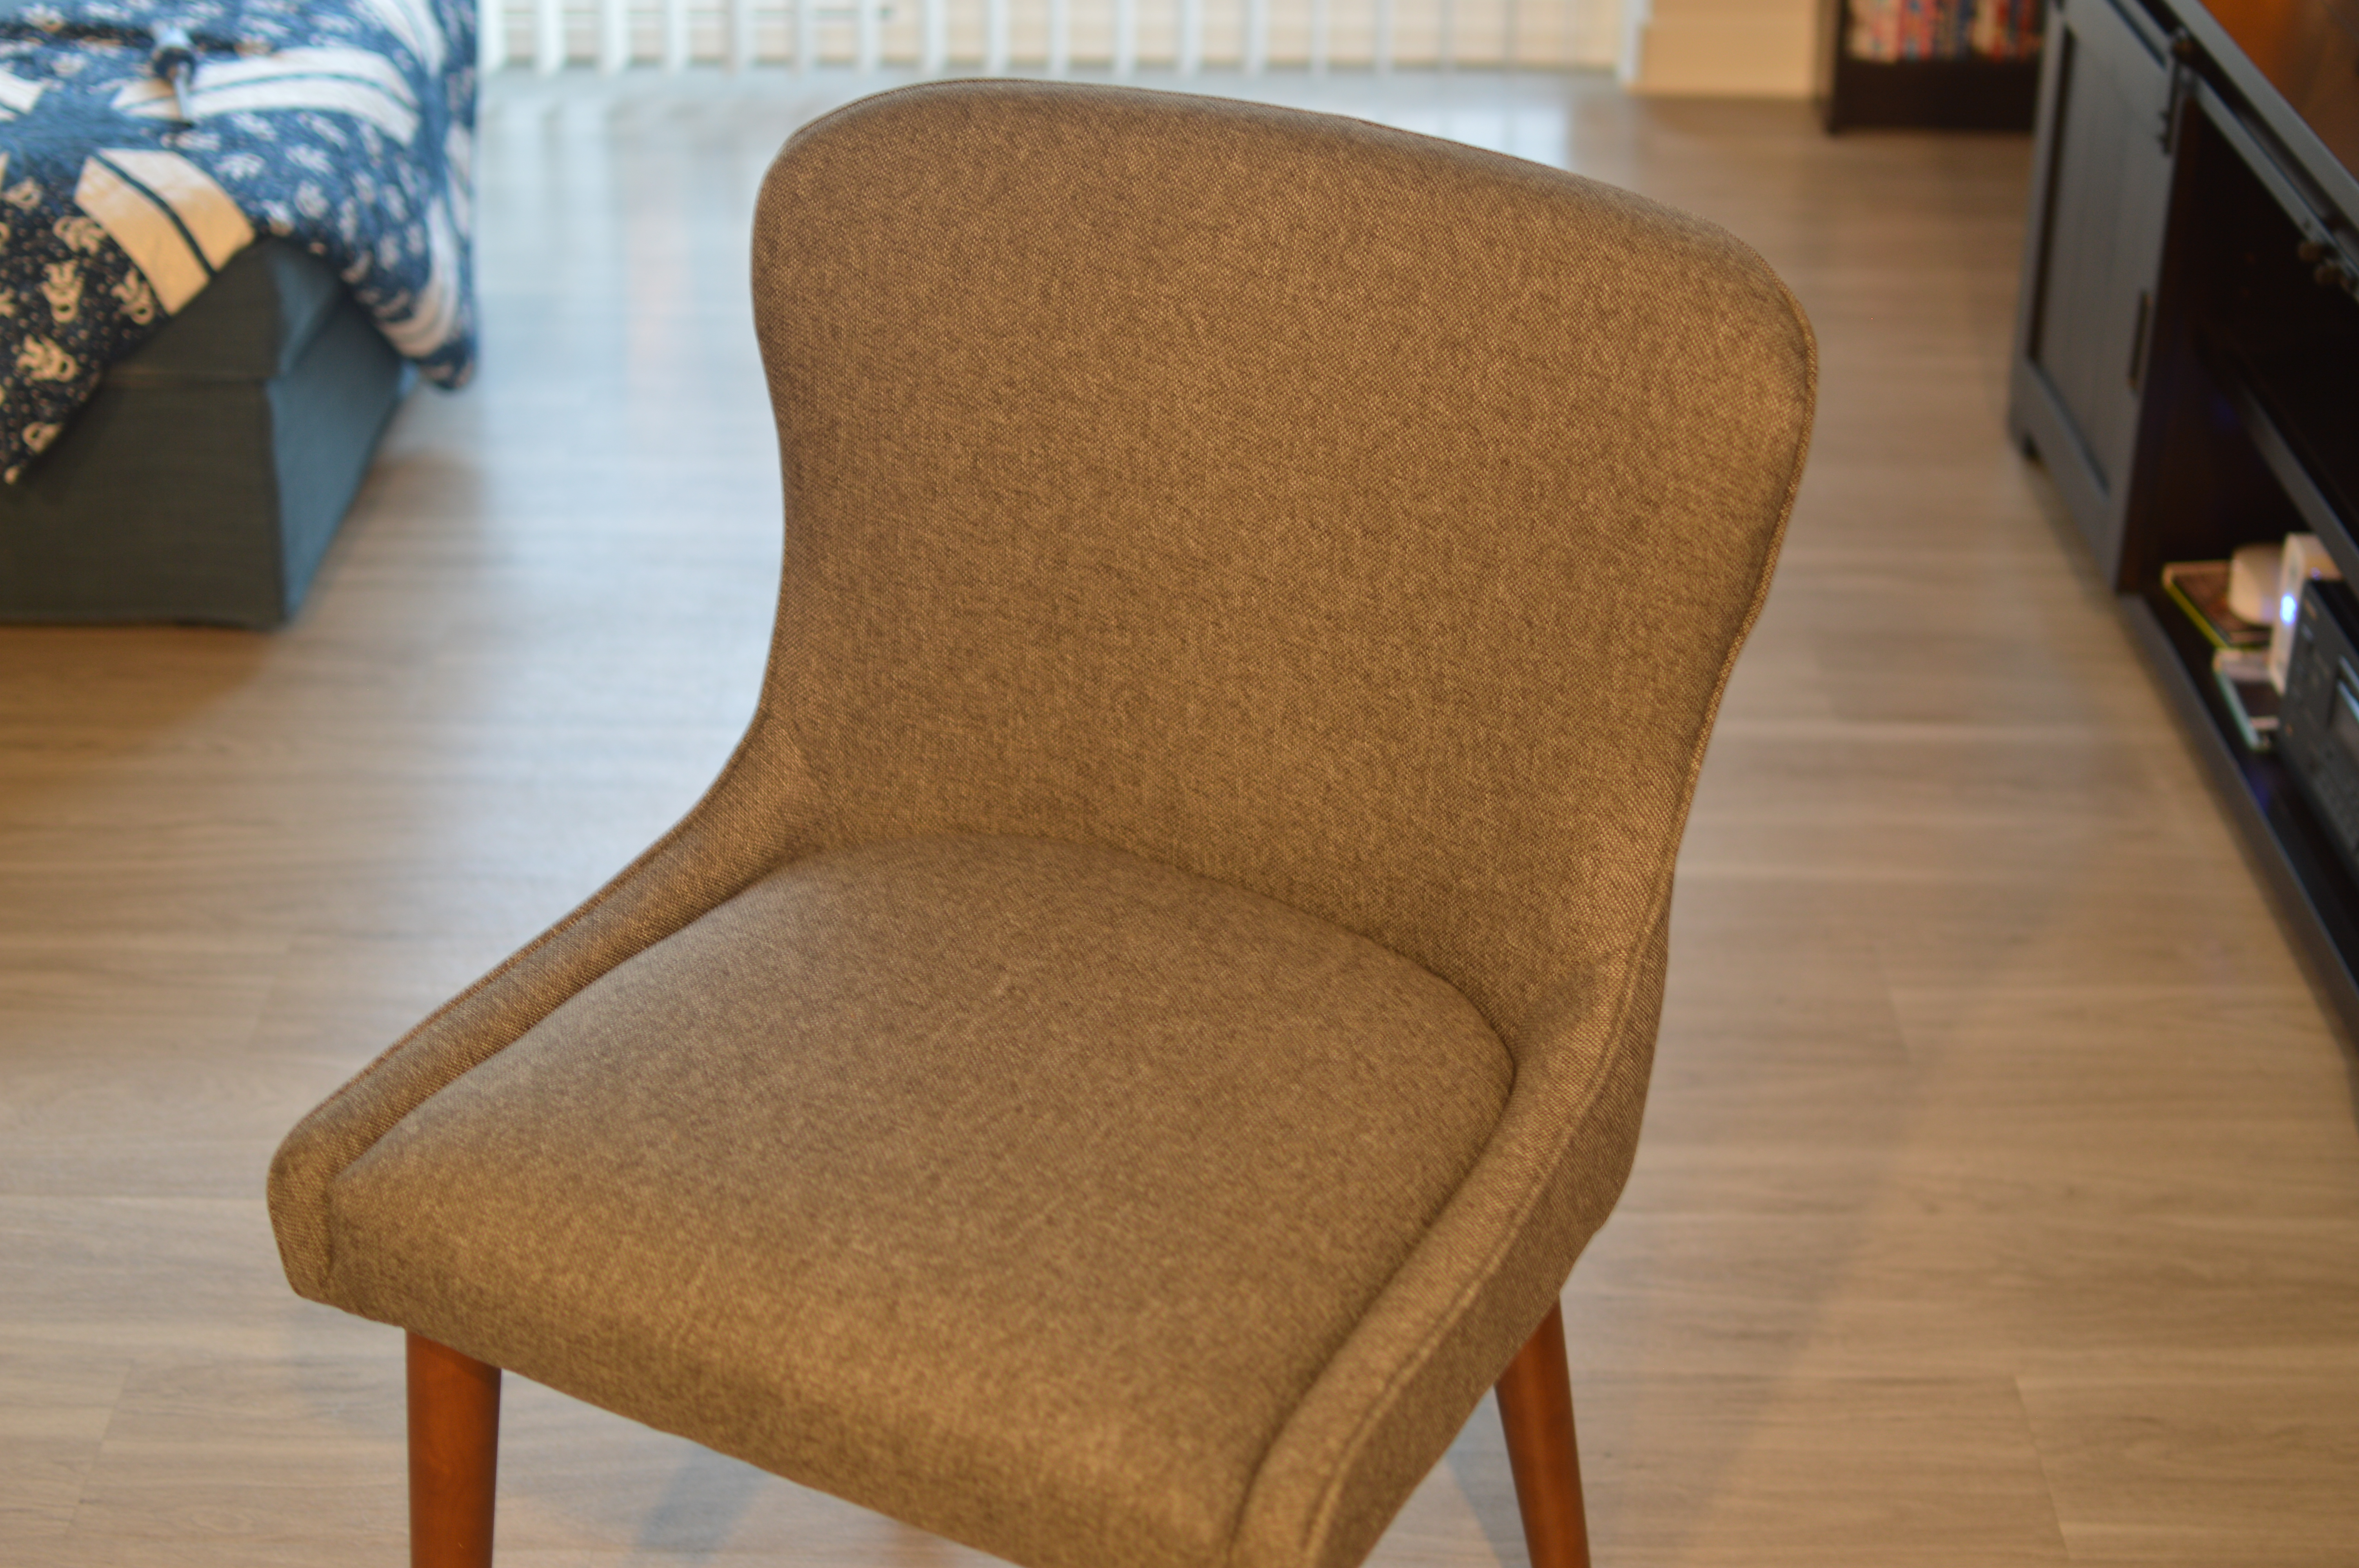
\includegraphics[width=0.95\textwidth]{Chair.JPG}
        \caption{}
        \label{fig:Chair}
    \end{subfigure}
    
    \caption{Backgrounds used in the BOS experiments including (a) an IKEA chair footrest, (b) a lamp shade, (c) a blanket, and (d) a chair.}
    \label{fig:Backgrounds}
\end{figure}

The backgrounds used are a footrest from my IKEA chair, a lamp shade, a blanket, and a normal chair.  These are all chosen because they have good small-scale structure that allows us to see small shifts in the pattern.  If you look around your apartment/house, you'll be able to find a bunch of things that can provide a nice background pattern.  Worst case scenario, you can print out a background of essentially TV static/noise on a piece of paper and use that as a background.  Background structure and size is an important part of designing a BOS experiment, so I won't be going into details here.  Just find something with small-scale structure and you should be fine.  The IKEA chair footrest is a little tougher than the rest because it is darker in color, so it needs more illumination to get the contrast we need.  The lamp shade is nice because it is back-illuminated by the LED bulb, meaning contrast is great.  The blanket and chair are both light in color, and provide a good background providing that it's daytime or you have decent light in the room.

% FIGURE: Cameras
\begin{figure}[h]
    \centering
    \begin{subfigure}[b]{0.35\textwidth}
    	\centering
        \includegraphics[height=3cm]{DSLR.JPG}
        \caption{}
        \label{fig:DSLR}
    \end{subfigure}
    \begin{subfigure}[b]{0.35\textwidth}
    	\centering
        \includegraphics[height=3cm]{Samsung_S6.JPG}
        \caption{}
        \label{fig:Samsung_S6}
    \end{subfigure}

    \caption{Cameras used in BOS experiments including (a) a Nikon D3200 DSLR and (b) a Samsung S6 phone.}
    \label{fig:Cameras}
\end{figure}

The two cameras I'm using are my Nikon D3200 DSLR and my Samsung S6 phone.  I use the DSLR camera for most of the experiments because I like taking picture and videos with it, and I have more control over the settings when using it.  I include the Samsung S6 to show you that you can get good BOS images with your phone as well, in case you don't have fancier camera.

% ------------------------------------
% ---- Candle: IKEA Chair: Candle ----
% ------------------------------------
\subsection{Candle: IKEA Chair: DSLR}
\label{subsec:Candle_IKEA_Chair_DSLR}

For the first test, I was using the IKEA chair footstool since it has a well defined small texture to it.  The only problem with this background is that it is dark, so it needs to be illuminated better than other backgrounds used later.  I placed a candle about half the distance from the camera to the background, and used my DSLR mounted on a tripod for these measurements.  By using a tripod, I avoid the need for the image registration step (Section \ref{subsec:Image_Registration}).  First, I make sure the camera is focused sharply on the background, then I start taking video without the candle in place, and then shortly after, I add the candle into the frame.  This means that I can get the background frame in the same video as the actual object frames.

% FIGURE: Python and MATLAB: Candle/IKEA Chair/DSLR
\begin{figure}[h]
    \centering
    \begin{subfigure}[b]{0.45\textwidth}
    	\centering
        \includegraphics[width=0.95\textwidth]{Python_Candle_Chair.PNG}
        \caption{}
        \label{fig:Python_Candle_Chair}
    \end{subfigure}
    \begin{subfigure}[b]{0.45\textwidth}
    	\centering
        \includegraphics[width=0.95\textwidth]{MATLAB_Candle_Chair.PNG}
        \caption{}
        \label{fig:MATLAB_Candle_Chair}
    \end{subfigure}

    \caption{BOS total displacement signal for a candle using my IKEA footrest as a background when processed by (a) Python and (b) MATLAB.}
    \label{fig:Candle_Chair}
\end{figure}

When processing the data, I used a window/search size of $8$/$16$.  Any smaller and the background becomes too noisy and starts to overshadow the actual BOS signal.  To see the difference the sub-pixel resolution makes for these images, see Section \ref{subsec:Study_Sub_Pixel_Resolution}.  The background looks slightly noisy here because I was just using the natural light in the room, as opposed to shining a light directly onto the background to increase the contrast and brightness.

% ----------------------------------------
% ---- Candle: Lamp Shade: Samsung S6 ----
% ----------------------------------------
\subsection{Candle: Lamp Shade: Samsung S6}
\label{subsec:Candle_Lamp_Shade_Samsung_S6}

For every other image/video in this document, I use my DSLR camera since it's easier to mount and easier to control in terms of its settings.  However, I recognize that not everyone has a DSLR camera, so in this section I'll show how you can also simply use your phone to get nice BOS results.  I'm imaging a candle with the lamp shade as the background.  I have my phone attached to a tripod so that I don't need to perform the time-consuming image registration.  The resulting BOS signal after processing through my Python code can be seen in Fig. \ref{fig:Candle_Light_Shade_Samsung_0p08_1p25}.

% FIGURE: Python and MATLAB, lighter both pre- and post-ignition, DSLR
\begin{figure}[h]
    \centering
	\includegraphics[height=5cm]{Candle_Light_Shade_Samsung_0p08_1p25.PNG}
    \caption{BOS total displacement signal for a candle using the lamp shade as the background when processed by Python.}
    \label{fig:Candle_Light_Shade_Samsung_0p08_1p25}
\end{figure}

While the pixel resolution of the videos I take on my phone are the same as the DSLR, sometimes my phone does auto-adjustments in the video itself, and this will affect the final BOS signal.  For example, in my DSLR BOS images, the backgrounds are generally all at the same pixel displacements (even though they may not be perfectly zero all the time).  Here, however, we can see that the background looks like it has a gradient.  At the bottom left, the displacements are small, as we would expect.  But as we look toward the top of the image, the displacements increase, even away from where we would expect them to (the plume above the flame).  This is potentially due to some auto-adjustment from my phone while I was filming.  You can still get nice BOS images from your phone, but just make sure to limit or disable any automatic adjustments to zoom/focus/etc. when you take your photos or videos.

% -----------------------------------
% ---- Lighter: Lamp Shade: DSLR ----
% -----------------------------------
\subsection{Lighter: Lamp Shade: DSLR}
\label{subsec:Lighter_Lamp_Shade_DSLR}

Now we'll use the same background we had in the previous section (the lamp shade), but now we will look at the lighter using my DSLR camera, also mounted on a tripod.  There are two sets of images here.  The first is the spurt of butane before ignition (Figs. \ref{fig:Python_PreLighter_DSLR} and \ref{fig:MATLAB_PreLighter_DSLR}), and the second is after the lighter has been ignited (Figs. \ref{fig:Python_PostLighter_DSLR} and \ref{fig:MATLAB_PostLighter_DSLR}).  I also have a video showing conventional schlieren (single-mirror, double-pass) of the ignition of the lighter fluid at $4000$ frames per second \cite{JTE_Lighter}.

% FIGURE: Python and MATLAB, lighter both pre- and post-ignition, DSLR
\begin{figure}[h]
    \centering
    \begin{subfigure}[b]{0.45\textwidth}
    	\centering
        \includegraphics[width=0.95\textwidth]{Python_LighterFluid.PNG}
        \caption{}
        \label{fig:Python_PreLighter_DSLR}
    \end{subfigure}
    \begin{subfigure}[b]{0.45\textwidth}
    	\centering
        \includegraphics[width=0.95\textwidth]{MATLAB_LighterFluid.PNG}
        \caption{}
        \label{fig:MATLAB_PreLighter_DSLR}
    \end{subfigure}
    
	\begin{subfigure}[b]{0.45\textwidth}
    	\centering
        \includegraphics[width=0.95\textwidth]{Python_Lighter_DSLR.PNG}
        \caption{}
        \label{fig:Python_PostLighter_DSLR}
    \end{subfigure}
    \begin{subfigure}[b]{0.45\textwidth}
    	\centering
        \includegraphics[width=0.95\textwidth]{MATLAB_Lighter_DSLR.PNG}
        \caption{}
        \label{fig:MATLAB_PostLighter_DSLR}
    \end{subfigure}
	
    \caption{BOS signal for (a,b) a spurt of butane pre-ignition and (c,d) the lighter post-ignition, using both (a,c) Python and (b,d) MATLAB.}
    \label{fig:Lighter_Fluid}
\end{figure}

% -----------------------------------
% ---- Blow Dryer: Blanket: DSLR ----
% -----------------------------------
\subsection{Blow Dryer: Blanket: DSLR}
\label{subsec:Blow_Dryer_Blanket_DSLR}

I have a light-gray blanket that looked like it could provide a good background, so I decided to try it with a hand-held blow dryer.  Note that these are images, not videos, so the resolution is better.  The window/search size was $16$/$32$ for this case, which was more than small enough since again, the resolution is better than the normal videos I would take.  The blow dryer processed with both Python and MATLAB can be seen in Figs. \ref{fig:Python_Blow_Dryer} and \ref{fig:MATLAB_Blow_Dryer}, respectively.

% FIGURE: Python tea lamp shade overlay
\begin{figure}[h]
    \centering
    \begin{subfigure}[b]{0.45\textwidth}
    	\centering
        \includegraphics[width=0.95\textwidth]{Python_Hairdryer.PNG}
        \caption{}
        \label{fig:Python_Blow_Dryer}
    \end{subfigure}
    \begin{subfigure}[b]{0.45\textwidth}
    	\centering
        \includegraphics[width=0.95\textwidth]{MATLAB_Hairdryer.PNG}
        \caption{}
        \label{fig:MATLAB_Blow_Dryer}
    \end{subfigure}

    \caption{BOS $X$-displacement signal for a blow dryer using a blanket as the background when processed by (a) Python and (b) MATLAB.}
\end{figure}

If you looked at the figure caption, you'll note that we are plotting the $X$-displacement in this case.  Even if I hadn't mentioned it, you would still be able to make an educated guess.  The blow dryer is pointed up, so we know that the air to the left and right of it should be (relatively) undisturbed.  That means we should be seeing a gradient from left to right, and no gradient from bottom to top.  This rules out a $Y$-displacement plot, but not a total displacement plot.  For that, look at the colors in the plot.  We have both low (dark purple and dark blue) and high (yellow and red) values across the blow dryer.  That means that we have negative and positive displacements.  If we were plotting total displacement, both the left and right edges of the blow dryer plume would be the same color (if the plume is axisymmetric, which it pretty much is).  That's actually what we can see in Figs. \ref{fig:Python_Candle_Chair} and \ref{fig:MATLAB_Candle_Chair}, where we are plotting total displacement.

% -------------------------------
% ---- Tea: Lamp Shade: DSLR ----
% -------------------------------
\subsection{Tea: Lamp Shade: DSLR}
\label{subsec:Tea_Lamp_Shade_DSLR}

After making myself a hot cup of tea, I figured we could try to see if we could see some signal using the lamp shade from before.  My DSLR was again placed on a tripod and I focused on the background.  I started recording, and then introduced the cup of tea approximately halfway between the camera and the lamp shade.

% FIGURE: Python tea lamp shade overlay
\begin{figure}[h]
    \centering
    \begin{subfigure}[b]{0.45\textwidth}
    	\centering
        \includegraphics[width=0.95\textwidth]{Python_Tea.PNG}
        \caption{}
        \label{fig:Python_Tea}
    \end{subfigure}
    \begin{subfigure}[b]{0.45\textwidth}
    	\centering
        \includegraphics[width=0.95\textwidth]{MATLAB_Tea.PNG}
        \caption{}
        \label{fig:MATLAB_Tea}
    \end{subfigure}

    \caption{BOS signal for tea using a lamp shade as the background when processed by (a) Python and (b) MATLAB.}
    \label{fig:Tea}
\end{figure}

The results in Figs. \ref{fig:Python_Tea} and \ref{fig:MATLAB_Tea} are for the same image processed in Python and MATLAB, respectively.  We can see in both images the nice BOS signal, but also that there is noise at both edges of the image.  This is because the lamp shade is cylindrical, and at the edges the image was out of focus since I was focusing on the front of the lamp shade.  This means we get erroneous displacements in these regions.  However, the BOS signal near the tea cup shows that we can get very small displacements using this method.

% -------------------------------------
% ---- Study: Sub-Pixel Resolution ----
% -------------------------------------
\subsection{Study: Sub-Pixel Resolution}
\label{subsec:Study_Sub_Pixel_Resolution}

Here, we will take a look at the difference between pixel resolution and sub-pixel resolution.  I'll be using the data from the PIV test case because it shows the effect most clearly.  The equation for a three-point Gaussian sub-pixel resolution can be found, for example, in the paper by Nobach and Honkanen \cite{2005_Nobach_EIF}.  The equation must be applied to both dimensions (row and column) of the cross-correlation map (denoted by $Z$).  For example, the sub-pixel shift from the maximum row index is given in Eq. \eqref{eq:Sub_Pixel_Row}.  The subscript $i$ refers to the row index of the peak/maximum of the cross-correlation surface.

\begin{equation}
\Delta r = \frac{\ln\left(Z_{i-1}\right)-\ln\left(Z_{i+1}\right)}{2\ln\left(Z_{i+1}\right) - 4\ln\left(Z_i\right) + 2\ln\left(Z_{i-1}\right)}
\label{eq:Sub_Pixel_Row}
\end{equation}

\noindent Similarly, the sub-pixel shift from the maximum column index is given in Eq. \eqref{eq:Sub_Pixel_Column}.  The subscript $j$ refers to the column index of the peak/maximum of the cross-correlation surface.

\begin{equation}
\Delta c = \frac{\ln\left(Z_{j-1}\right)-\ln\left(Z_{j+1}\right)}{2\ln\left(Z_{j+1}\right) - 4\ln\left(Z_j\right) + 2\ln\left(Z_{j-1}\right)}
\label{eq:Sub_Pixel_Column}
\end{equation}

\noindent If the index peak (ip) of the cross-correlation surface is given by $r_\text{ip}$ for the maximum row index and by $c_\text{ip}$ for the maximum column index, then we can write the final sub-pixel peak (spp) of the cross-correlation map as seen in Eq. \eqref{eq:Sub_Pixel}.

\begin{equation}
\begin{aligned}
r_\text{ssp} &=& r_\text{ip} + \Delta r \\
c_\text{ssp} &=& c_\text{ip} + \Delta c
\end{aligned}
\label{eq:Sub_Pixel}
\end{equation}

% FIGURE: Sub-pixel resolution comparison using PIV test case
\begin{figure}[h]
    \centering
    \begin{subfigure}[b]{0.35\textwidth}
    	\centering
        \includegraphics[width=0.95\textwidth]{Sub_Pixel_No_PIV.PNG}
        \caption{}
        \label{fig:Sub_Pixel_No_PIV}
    \end{subfigure}
    \begin{subfigure}[b]{0.35\textwidth}
    	\centering
        \includegraphics[width=0.95\textwidth]{Sub_Pixel_Yes_PIV.PNG}
        \caption{}
        \label{fig:Sub_Pixel_Yes_PIV}
    \end{subfigure}

    \caption{Comparison of PIV test case images (a) without sub-pixel resolution and (b) with sub-pixel resolution.}
    \label{fig:Sub_Pixel_Resolution}
\end{figure}

The window/search sizes are $8$/$16$ with a threshold of $5$, and I'm plotting the total displacement.  For both the pixel and sub-pixel resolution cases, I am using $0$ to $6$ as the colormap bounds.  The resulting BOS signals without and with sub-pixel resolution can be seen in Figs. \ref{fig:Sub_Pixel_No_PIV} and \ref{fig:Sub_Pixel_Yes_PIV}, respectively.  The image with sub-pixel resolution looks much better, even though we can see the same solution structure in the image without sub-pixel resolution.  It is easier to tell from Fig. \ref{fig:Sub_Pixel_Yes_PIV} that this flow is a rotational flow about a center point.  Using sub-pixel resolution also significantly helps when using images where displacements are small and image resolution isn't so great.  I use sub-pixel resolution for all the results shown in this document.

% ---------------------------------------
% ---- Study: Distance to Background ----
% ---------------------------------------
\subsection{Study: Distance to Background}
\label{subsec:Study_Distance_to_Background}

How far should you place your object from the background?  Generally, it depends.  But in this section I'll show you how the results change for different object-to-background distances, and you can play around with it yourself as well.  I'm using the back of a chair to image a candle with my DSLR.  The candle was placed near the chair, half-way between the chair and the camera, and near the camera.

% FIGURE: Sub-pixel resolution comparison using PIV test case
\begin{figure}[h]
    \centering
    \begin{subfigure}[b]{0.3\textwidth}
    	\centering
        \includegraphics[width=0.95\textwidth]{Study_BGDist_Far.JPG}
        \caption{}
        \label{fig:Study_BGDist_Far}
    \end{subfigure}
    \begin{subfigure}[b]{0.3\textwidth}
    	\centering
        \includegraphics[width=0.95\textwidth]{Study_BGDist_Mid.JPG}
        \caption{}
        \label{fig:Study_BGDist_Mid}
    \end{subfigure}
    \begin{subfigure}[b]{0.3\textwidth}
    	\centering
        \includegraphics[width=0.95\textwidth]{Study_BGDist_Near.JPG}
        \caption{}
        \label{fig:Study_BGDist_Near}
    \end{subfigure}
    
	\begin{subfigure}[b]{0.3\textwidth}
    	\centering
        \includegraphics[height=5cm]{BGDist_Far_0_1.PNG}
        \caption{}
        \label{fig:BOS_BGDist_Far}
    \end{subfigure}
    \begin{subfigure}[b]{0.3\textwidth}
    	\centering
        \includegraphics[height=5cm]{BGDist_Mid_0_2p5.PNG}
        \caption{}
        \label{fig:BOS_BGDist_Mid}
    \end{subfigure}
    \begin{subfigure}[b]{0.3\textwidth}
    	\centering
        \includegraphics[height=5cm]{BGDist_Near_0_3p5.PNG}
        \caption{}
        \label{fig:BOS_BGDist_Near}
    \end{subfigure}
    
    \caption{Comparison of BOS data using three placement locations of the object (candle): (a,d) close to the background, (b,e) between background and camera, and (c,f) close to the camera.}
    \label{fig:Study_BGDist}
\end{figure}

For this particular test, I was using an f/\# of $1.8$, exposure of $1/50$, ISO of $100$, and my $35$ mm prime lens.  This is an extremely low f/\# to be using, which is why the candle gets blurrier as I move it closer to the camera.  I was using this wide aperture size so I could get a faster shutter to freeze the motion, but generally you would want to decrease the aperture size to get a deeper depth of field (increase the f/\#).  For experiments at home, just do whatever will give you your best results.

From the results shown in Figs. \ref{fig:BOS_BGDist_Far}, \ref{fig:BOS_BGDist_Mid}, and \ref{fig:BOS_BGDist_Near}, we can see the candle flame is sharpest when it is closest to the background, which is where we are focusing the camera.  However, the displacements are smaller (using colormap limits from $0$ to $1$ for Fig. \ref{fig:BOS_BGDist_Far}).  When we place the candle midway between the background and the camera, the flame is more out-of-focus, but the displacements are larger (colormap limits from $0$ to $2.5$ for Fig. \ref{fig:BOS_BGDist_Mid}).  The region of the image that is occupied by actual displacements becomes larger as we move the candle towards the camera, because it is physically taking up more of the field of view of the camera.

% ----------------------------
% ---- Study: F/# Changes ----
% ----------------------------
\subsection{Study: f/\# Changes}
\label{subsec:Study_F_Number_Changes}

Now we can look at how the f/\# changes the BOS signal we see.  I'm using four different values: f/$1.8$, f/$5$, f/$10$, and f/$20$.  The setup is the same as the previous section (Section \ref{subsec:Study_Distance_to_Background}), where the candle is placed midway between the background (chair-back) and camera (DSLR).

% FIGURE: Study: F/# Changes
\begin{figure}[h]
    \centering
    \begin{subfigure}[b]{0.35\textwidth}
    	\centering
        \includegraphics[height=5cm]{FNumber_1p8_0_2.PNG}
        \caption{}
        \label{fig:FNumber_1p8_0_2}
    \end{subfigure}
    \begin{subfigure}[b]{0.35\textwidth}
    	\centering
        \includegraphics[height=5cm]{FNumber_5_0_2.PNG}
        \caption{}
        \label{fig:FNumber_5_0_2}
    \end{subfigure}
    
    \begin{subfigure}[b]{0.35\textwidth}
    	\centering
        \includegraphics[height=5cm]{FNumber_10_0_2.PNG}
        \caption{}
        \label{fig:FNumber_10_0_2}
    \end{subfigure}
    \begin{subfigure}[b]{0.35\textwidth}
    	\centering
        \includegraphics[height=5cm]{FNumber_20_0_2.PNG}
        \caption{}
        \label{fig:FNumber_20_0_2}
    \end{subfigure}

    \caption{BOS results for F/\# values of (a) $1.8$, (b) $5$, (c) $10$, and (d) $20$.}
    \label{fig:FNumber}
\end{figure}

The results for the four cases are shown in Fig. \ref{fig:FNumber}.  As the f/\# increases, the aperture decreases, the depth of field becomes larger, and the candle gets sharper.  All results use a window/search size of $16$/$32$, and the colormap limits for all images is $0$ to $2$.  While the results for the largest f/\# look quite good, note that it is not always desirable to shoot at such small apertures.  For a nice interactive explanation, see the Cambridge in Colour website \cite{Cambridge_in_Colour}.

% ------------------------------
% ---- Study: Interpolation ----
% ------------------------------
\subsection{Study: BOS Signal Interpolation}
\label{subsec:BOS_Signal_Interpolation}

In this section, we will see what happens when we interpolate the resulting BOS signal to a coarser, or finer grid.  The BOS signal results are dictated by the window and search sizes that are used in the analysis section of the codes.  However, one way to smooth coarse data a little is to use interpolation between the actual computed values.  In Fig. \ref{fig:Interpolation}, the total displacement for the PIV challenge images is shown.  The actual computed BOS signal is shown in Fig. \ref{fig:Interpolation_1}, where a window/search size of $8$/$16$ was used.

% FIGURE: Interpolation of resulting BOS signal: 0.25, 0.5, 1, and 2
\begin{figure}[h]
    \centering
    \begin{subfigure}[b]{0.35\textwidth}
    	\centering
        \includegraphics[width=0.95\textwidth]{Interpolation_0p25.PNG}
        \caption{}
        \label{fig:Interpolation_0p25}
    \end{subfigure}
    \begin{subfigure}[b]{0.35\textwidth}
    	\centering
        \includegraphics[width=0.95\textwidth]{Interpolation_0p5.PNG}
        \caption{}
        \label{fig:Interpolation_0p5}
    \end{subfigure}
    
    \begin{subfigure}[b]{0.35\textwidth}
    	\centering
        \includegraphics[width=0.95\textwidth]{Interpolation_1.PNG}
        \caption{}
        \label{fig:Interpolation_1}
    \end{subfigure}
    \begin{subfigure}[b]{0.35\textwidth}
    	\centering
        \includegraphics[width=0.95\textwidth]{Interpolation_2.PNG}
        \caption{}
        \label{fig:Interpolation_2}
    \end{subfigure}

    \caption{Comparison of PIV test case with interpolation BOS signals of (a) 0.25, (b) 0.5, (c) 1 (original solution), and (d) 2.}
    \label{fig:Interpolation}
\end{figure}

The solution is a little pixelated based on those computational parameters, so to smooth the data a little, we can apply a $2$-times interpolation, which just doubles the number of grid points in both the $X$ and $Y$ direction.  This is shown in Fig. \ref{fig:Interpolation_2}, where the signal looks the same, but the pixelation is not as clear anymore.  In a similar since (although there's no reason to do this), we can interpolate to a coarser grid, as seen in Figs. \ref{fig:Interpolation_0p25} and \ref{fig:Interpolation_0p5} for a quarter-grid and half-grid, respectively.  Note that this post-processing of the data does not increase the resolution of the actual computed data, it is merely interpolating the existing solution to grid points in between those that were actually solved for.  This is only used for visualization purposes.

% -----------------------------------
% ---- Study: More Advanced Code ----
% -----------------------------------
\subsection{Study: More Advanced Code}
\label{subsec:Study_More_Advanced_Code}

The code I have written is very basic.  It is not the most efficient way to write a cross-correlation BOS/PIV code.  It doesn't have all the bells and whistles that a better code would.  It was written such that it would be easy to use, and easy to edit if you want to add your own functionality.  A friend of mine ran the candle image through his more advanced PIV code, and we can look at those results in this section (from Section \ref{subsec:Candle_IKEA_Chair_DSLR}).

% FIGURE: More advanced code
\begin{figure}[h]
    \centering
	\includegraphics[height=5cm]{Tim_Candle.PNG}
    \caption{More advanced PIV algorithm for (a) the candle data from Section \ref{subsec:Candle_IKEA_Chair_DSLR} and (b) the tea data from Section \ref{subsec:Tea_Lamp_Shade_DSLR}.}
    \label{fig:Tim_Candle}
\end{figure}

%% FIGURE: More advanced code
%\begin{figure}[h]
%    \centering
%    \begin{subfigure}[b]{\textwidth}
%    	\centering
%        \includegraphics[height=5cm]{Tim_Candle.PNG}
%        \caption{}
%        \label{fig:Tim_Candle}
%    \end{subfigure}
%    
%    \begin{subfigure}[b]{\textwidth}
%    	\centering
%        \includegraphics[height=5cm]{Tim_Tea.PNG}
%        \caption{}
%        \label{fig:Tim_Tea}
%    \end{subfigure}
%
%    \caption{More advanced PIV algorithm for (a) the candle data from Section \ref{subsec:Candle_IKEA_Chair_DSLR} and (b) the tea data from Section \ref{subsec:Tea_Lamp_Shade_DSLR}.}
%    \label{fig:Tim}
%\end{figure}

The results for the candle can be seen in Fig. \ref{fig:Tim_Candle}, which is plotting the $X$-displacement.  These results look similar to the images from before, but the background is noticeably less noisy.  The test data I've taken at home is not a great way to see how much better the advanced code is.  It uses a better algorithm that, in essence, will deform the images such that much smaller displacements can be found without decreasing the window/search size and generating more noise in the data.  This method is referred to as the window displacement iterative mutligrid, or WIDIM \cite{2000_Scarano}.

% =============================
% ==== MISCELLANEOUS NOTES ====
% =============================
\section{Miscellaneous Notes}
\label{sec:Miscellaneous_Notes}

\begin{itemize}
\item If you get an error in Python that \textit{matplotlib} has an error, just re-install it with \textit{Conda} using the command \texttt{conda install matplotlib}.  Alternatively, if you have \textit{pip} installed, you can run \texttt{pip install matplotlib}.
\item The ImageJ macro I made exports in a certain format.  If you want it to output to something different, simply update the macro to do what you want.
\item I am not exploring the use of custom BOS backgrounds, such as those typically used in a laboratory setting.  This document simply goes through using backgrounds you can find around your house/apartment.
\item When running the code, there may be a warning/message that appears along the lines of ``I1\_Sub or I2\_Sub has the same values in entire matrix!''.  There's no need to worry.  This just means that the current window/search location is at the object that isn't moving, and has the same values in the entire window/search region.  This obviously won't give a displacement, which is what the warning is referencing.
\end{itemize}

% ======================
% ==== KNOWN ISSUES ====
% ======================
\section{Known Issues}
\label{sec:Known_Issues}

% -----------------------
% ---- MATLAB Issues ----
% -----------------------
\subsection{MATLAB Issues}
\label{subsec:MATLAB_Issues}

\begin{itemize}
\item When zooming in on the overlay plot, the transparency of the overlay does not work.  When fully zoomed back out, the transparency returns.
\item The left and top (first row and first column) of the data looks like it has values that are incorrect by a scalar.  If concerned about these edges, just ignore the first row and column.
\item If you realized you made a mistake in the settings and have already pressed \textit{Compute}, and you try to close out of the cropping selection window that has opened, an error will occur and the image that was just on the screen will appear ``burned'' into the GUI window.  I generally just restart the GUI if this happens.
\item Error handling for every possible mistake the user can make is not included.  If you get an error and you know why, either let me know, or just edit the code yourself to handle that error.
\item If the loaded file names are very long, they will run onto the next line in the GUI and get cut off.
\item The \textcolor{myBlue}{\textit{Number of Frames}} option in the \textbf{Video} section is always set to a default value of $5$ regardless of how many frames there are in the chosen directory.
\end{itemize}

% -----------------------
% ---- Python Issues ----
% -----------------------
\subsection{Python Issues}
\label{subsec:Python_Issues}

\begin{itemize}
\item There is no video sequence capability yet.
\item There is no interpolation option available yet.
\item Selecting regions in final BOS image to set colormap bounds is not implemented.
\end{itemize}

% ====================
% ==== REFERENCES ====
% ====================
\bibliographystyle{abbrv}
\bibliography{./DIY_BOS}


\end{document}